\newpage
\section{Results}\label{Sec:Results}

The results are presented in three parts that correspond to the three research questions put forward in Section~\ref{Sec:Intro;Subsec:Present}: First, the forecasting accuracy of the prediction models is evaluated and reported. Second, the results of the market simulation -- which was run once with the true consumption and production values and once with predicted consumption values in three different supply scenarios -- are presented. Third, the implications of the results of the market simulation are discussed.


%%%%%%%%%%%%%%%%%%%%%%%%%%%%
%%%   Benchmark models   %%%
%%%%%%%%%%%%%%%%%%%%%%%%%%%%

\subsection{Evaluation of the prediction models}\label{Sec:Results;Subsec:Forecast}

Three prediction methods were used to forecast the energy consumption of 88 consumer households and to forecast the energy production of 12 prosumer households 15 minutes ahead: a benchmark model (see Section~\ref{Sec:Method;Subsec:Benchmark}), a LSTM RNN model (see Section~\ref{Sec:Method;Subsec:LSTM}), and a LASSO model (see Section~\ref{Sec:Method;Subsec:LASSO}). All three prediction models were compared and evaluated using the error measures presented in Section~\ref{Sec:Method;Subsec:Error}.


%%%%%%%%%%%
\subsubsection{Consumption data}

The performance of the prediction models was tested on a quarter of the available data. That is, the prediction models were fitted on the consumption values from 01.01.2017~00:00 to 30.09.2017~00:00 which is equivalent to 131,040 data points per data set. For all 88 consumer data sets, the models were fitted separately resulting in as many distinct LASSO and LSTM prediction models. The fitted models were then used to make energy consumption predictions in 15-minutes intervals for each household individually on the data from 01.10.2017~00:00 to 01.01.2018~00:00. This equates to 8,836 predicted values per data set per prediction method.

Figure~\ref{Fig:glimpse_predcons} exemplary shows the true and predicted consumption values of consumer~011 on October 27, 2017. The na\"ive benchmark model just follows the true consumption shifted by one time step (i.e., 15 minutes). This fits the true values generally good, as long as there are no sudden jumps in the household's energy consumption. Spikes in energy consumption, as in this example one occurred in the 15 minutes before 07:30 a.m.~and 08.30 a.m.~respectively, necessarily lead to two periods with high errors of the na\"ive predictor: First, once the jump to a high consumption level occurs and the na\"ive predictor remains at the previous low level, and second, once the consumption suddenly returns to the low consumption level and the na\"ive predictor persists at the high level of the previous period. In such situations, the LASSO and LSTM models are more accurate. Even though they underestimate the jumps in energy consumption, they do not lag behind as much as the na\"ive predictor and, generally, have the ability to anticipate movements. However, the exemplary glimpse onto the predicted consumption values of consumer~011 already reveals that also the sophisticated prediction models lack the ability to accurately predict sudden movements in the energy consumption and tend to overestimate low consumption levels and underestimate spikes in energy consumption.
%
\begin{figure}[htbp]
    \centering
    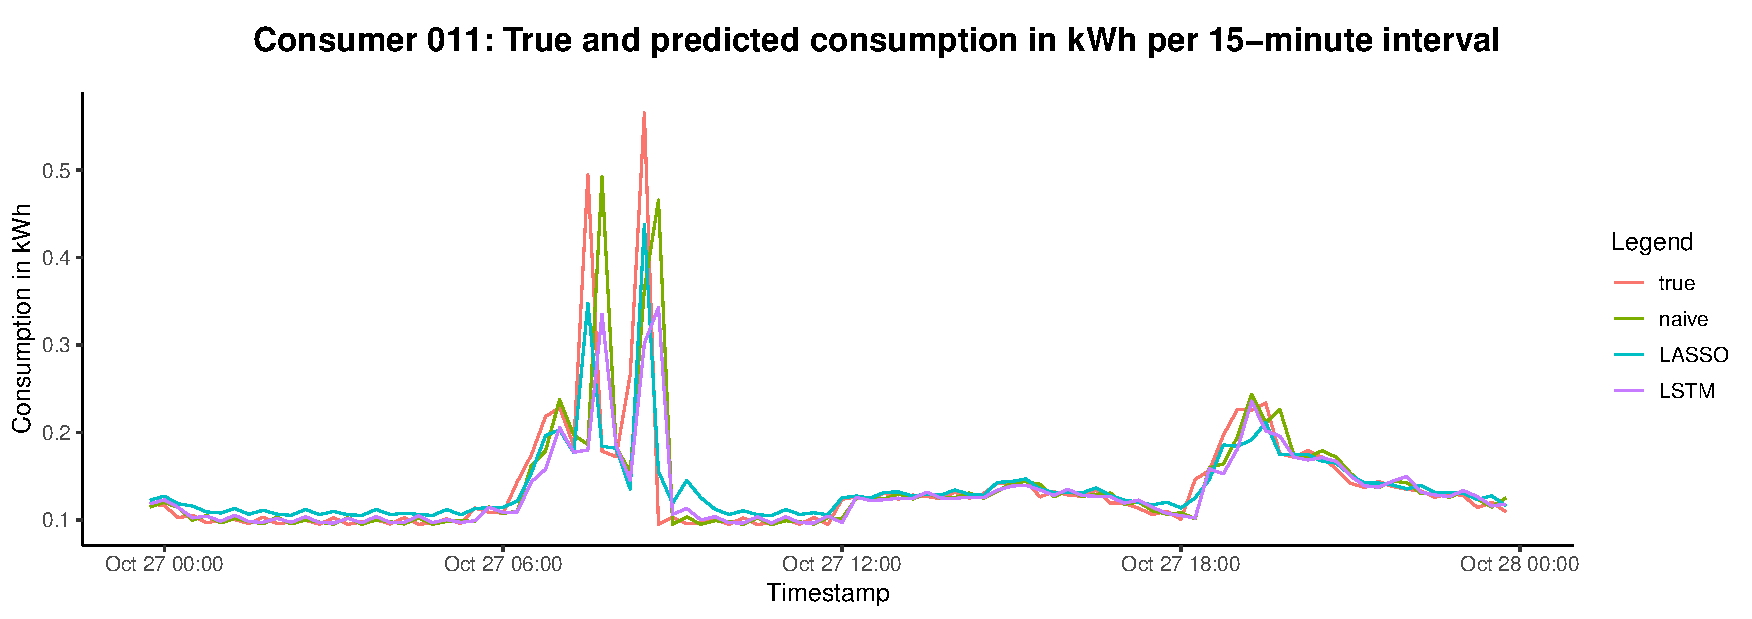
\includegraphics[width=\textwidth]{thesis/graphs/evaluation/c011_pred_cons.pdf}
    \caption[Exemplary 24 hours of true and predicted consumption values]{Exemplary 24 hours of true and predicted consumption values of consumer 011. \quantnet\href{https://github.com/QuantLet/BLEM/tree/master/BLEMplotEnergyPreds}{BLEMplotEnergyPreds}}
    \label{Fig:glimpse_predcons}
\end{figure}
%

Systematically analyzing the total over- and underestimation of the different prediction models on each consumer data set confirms this impression. Figure~\ref{Fig:overunderestimation} displays the total sum of over- and underestimation errors of each prediction method per data set. As one would expect, the na\"ive benchmark model consistently over- and underestimated by the same amount per data set. The reason for that is that the sum of over- and underestimation errors only depends on the amplitude of the spikes in energy consumption. Thus, overestimation errors occur in the same frequency and magnitude as underestimation errors. The LASSO model achieved overall lower total sums of errors than the benchmark model. Notably, the sum of underestimation errors is higher across the data sets than the sum of overestimation errors. This points towards a general tendency of underestimating sudden increases in energy consumption by the LASSO model.
%
\begin{figure}[!ht]
    \centering
    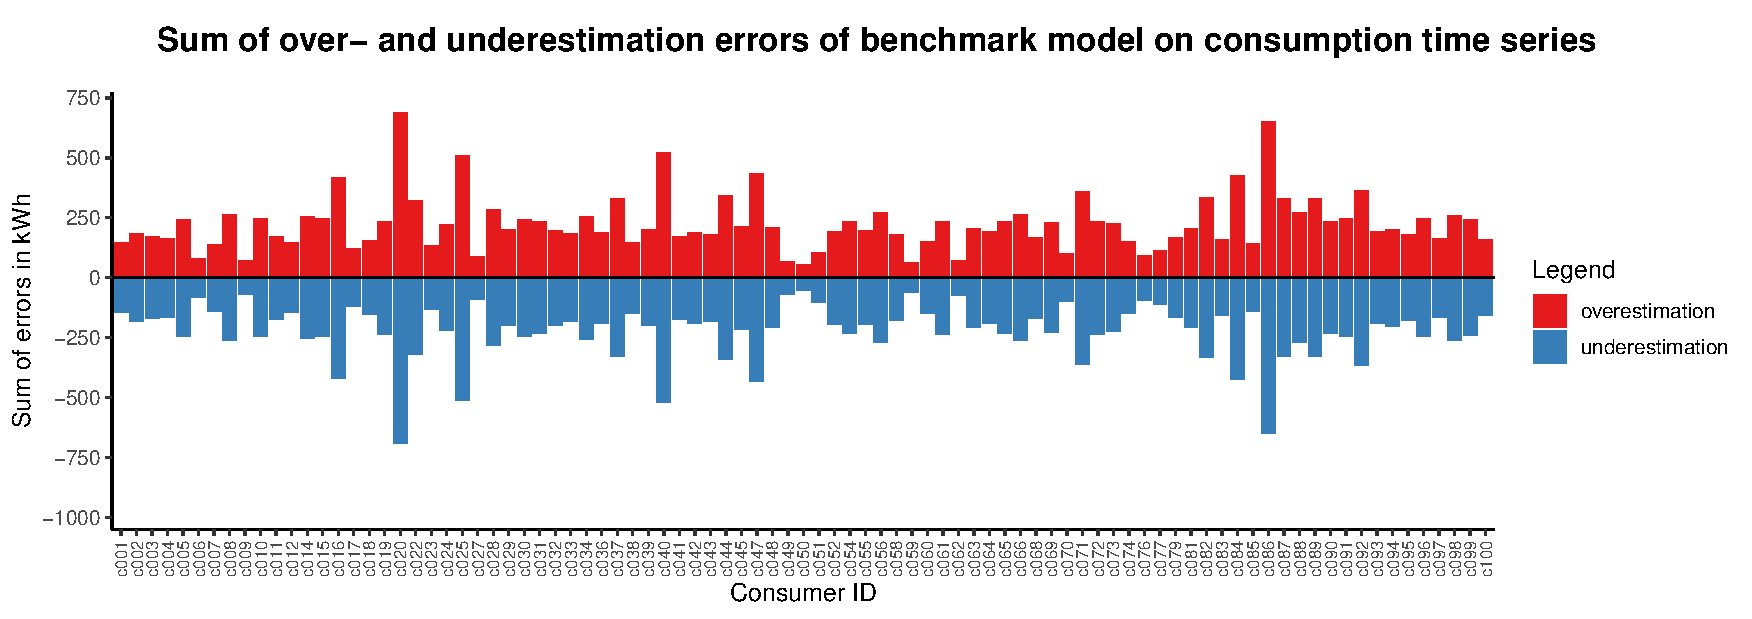
\includegraphics[width=\textwidth]{thesis/graphs/evaluation/c_barplot_naive_overunderestimation.pdf}\\\vspace{.6cm}
    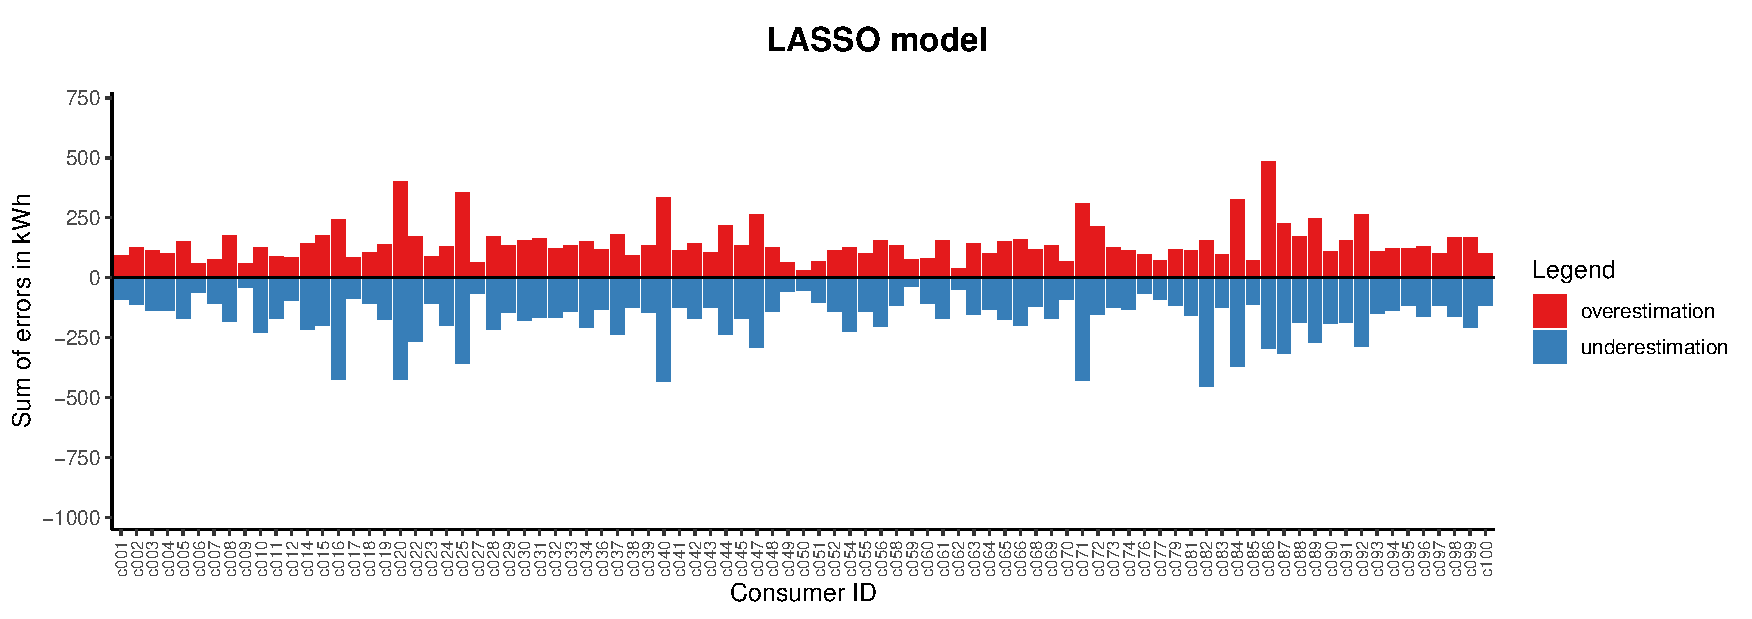
\includegraphics[width=\textwidth]{thesis/graphs/evaluation/c_barplot_LASSO_overunderestimation.pdf}\\\vspace{.6cm}
    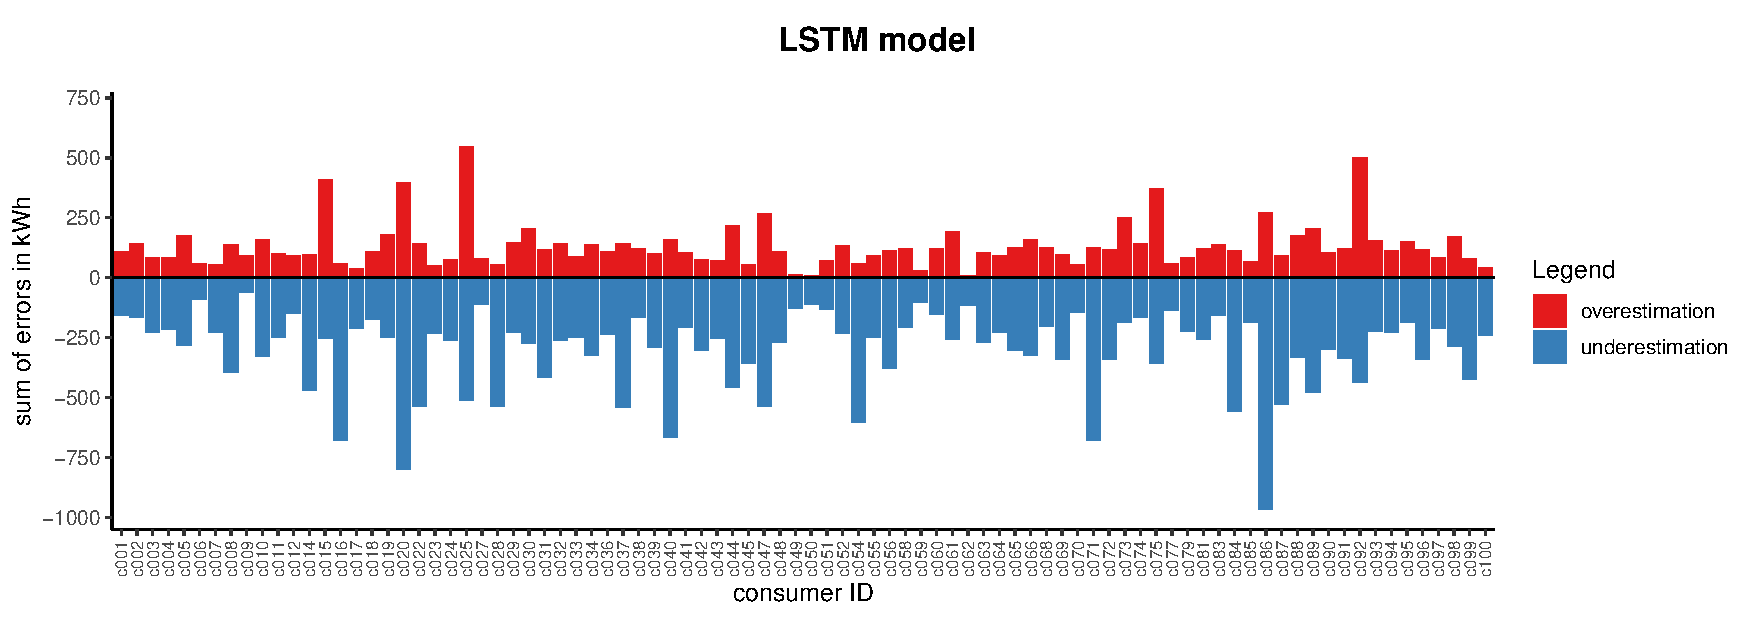
\includegraphics[width=\textwidth]{thesis/graphs/evaluation/c_barplot_LSTM_overunderestimation.pdf}
    \caption[Sum of total over- and underestimation errors per consumer data set]{Sum of total over- and underestimation errors of energy consumption per consumer data set and prediction model. \quantnet\href{https://github.com/QuantLet/BLEM/tree/master/BLEMplotPredErrors}{BLEMplotPredErrors}}
    \label{Fig:overunderestimation}
\end{figure}
%

The LSTM model on the other hand shows a much higher variability in the sums of over- and underestimation errors. By tendency, the overestimation errors of the LSTM model were smaller than those of the LASSO and benchmark models. Nevertheless, the underestimation is much more pronounced in the case of the LSTM model. Especially, some data sets stand out regarding the high sum of underestimation errors. This points towards a much higher heterogeneity in the suitability of the LSTM model to predict consumption values depending on the energy consumption pattern of the specific data set. The LASSO model on the other hand seems to be more equally well suited for all data sets and their particular consumption patterns.


The average performance of the three prediction models across all 88 data sets is shown in Table~\ref{Tab:avg_errormeasures}. As can be seen, LASSO and LSTM consistently outperformed the benchmark model according to MAE, RMSE, MAPE, and MASE. Interestingly, due to the heavy penalty NRMSE puts on comparably large prediction errors, both sophisticated prediction methods perform worse according to NRMSE, however.
%
\begingroup\catcode`"=9
\begin{table}[htbp]
{\footnotesize
    \csvreader[centered tabular=l|SSSSS,
    before reading=\sisetup{round-mode=places,round-precision=2,round-integer-to-decimal},
    filter not strcmp={\thecsvinputline}{1},
    table head=
    \hline\hline
     \multicolumn{1} {l}{\textbf{Model}} & \multicolumn{1} {c}{\textbf{MAE}} & \multicolumn{1} {c}{\textbf{RMSE}} & \multicolumn{1} {c}{\textbf{MAPE}} & \multicolumn{1} {c}{\textbf{NRMSE}} & \multicolumn{1} {c}{\textbf{MASE}}\\
    \hline,
    no head,
    separator=comma,
    respect all,
    late after line=\\,
    table foot=\hline \hline]
    {thesis/tables/avg_errorMeasures_c.csv}{}%
    {\csvcolii & \csvcoliii & \csvcoliv & \csvcolv & \csvcolvi & \csvcolvii}}%
    \caption[Mean of error measures for prediction on consumer data sets]{Mean of error measures for the prediction of energy consumption across all 88 consumer data sets. \quantnet\href{https://github.com/QuantLet/BLEM/tree/master/BLEMevaluateEnergyPreds}{BLEMevaluateEnergyPreds}}
    \label{Tab:avg_errormeasures}
\end{table}
\endgroup
%

A detailed analysis of this unexpected result reveals that it is mainly driven by an extremely bad NRMSE score for LSTM and LASSO on merely one out of the 88 data sets. As can be seen in Figure~\ref{Fig:heatmaps}, the predictions on consumer data set 027 have a particularly high NRMSE (and MAPE) compared to all other data sets. However, this pattern is not present in the absolute error measures. Further investigating the prediction errors of the forecasts on consumer 027 exposes that the high NRMSE score is driven by merely one observations: Between 24.11.2017 11:30 and 11:45 the energy consumption falls below 3 $\times$ $10^{-6}$. Due to this true value, $x_t$, which is very close to zero, the relative squared error $e_t = \left(\frac{\widehat{x}_t-x_t}{x_t}\right)^2$ is extremely high (see Appendix~\hyperlink{AppA4:Figures:erroranalysis}{A4}). This single extreme relative error pushes the NRMSE of the LSTM predictions to the staggering value of $\text{NRMSE}_{c027}=2383.46$. The same is true for MAPE, although not as extreme.
%
\begin{figure}[!ht]
 \centering
 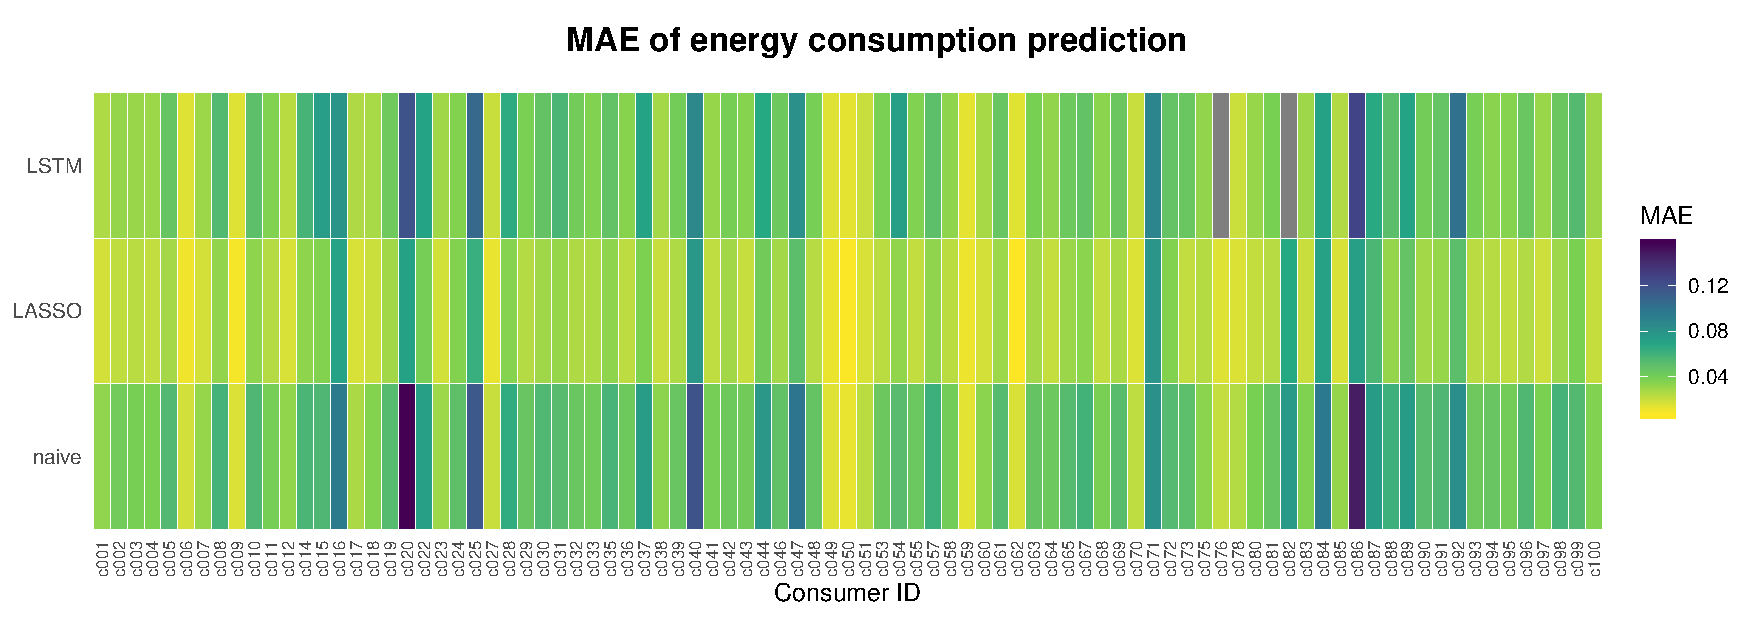
\includegraphics[width=\textwidth]{thesis/graphs/evaluation/c_heatmap_MAE.pdf}
 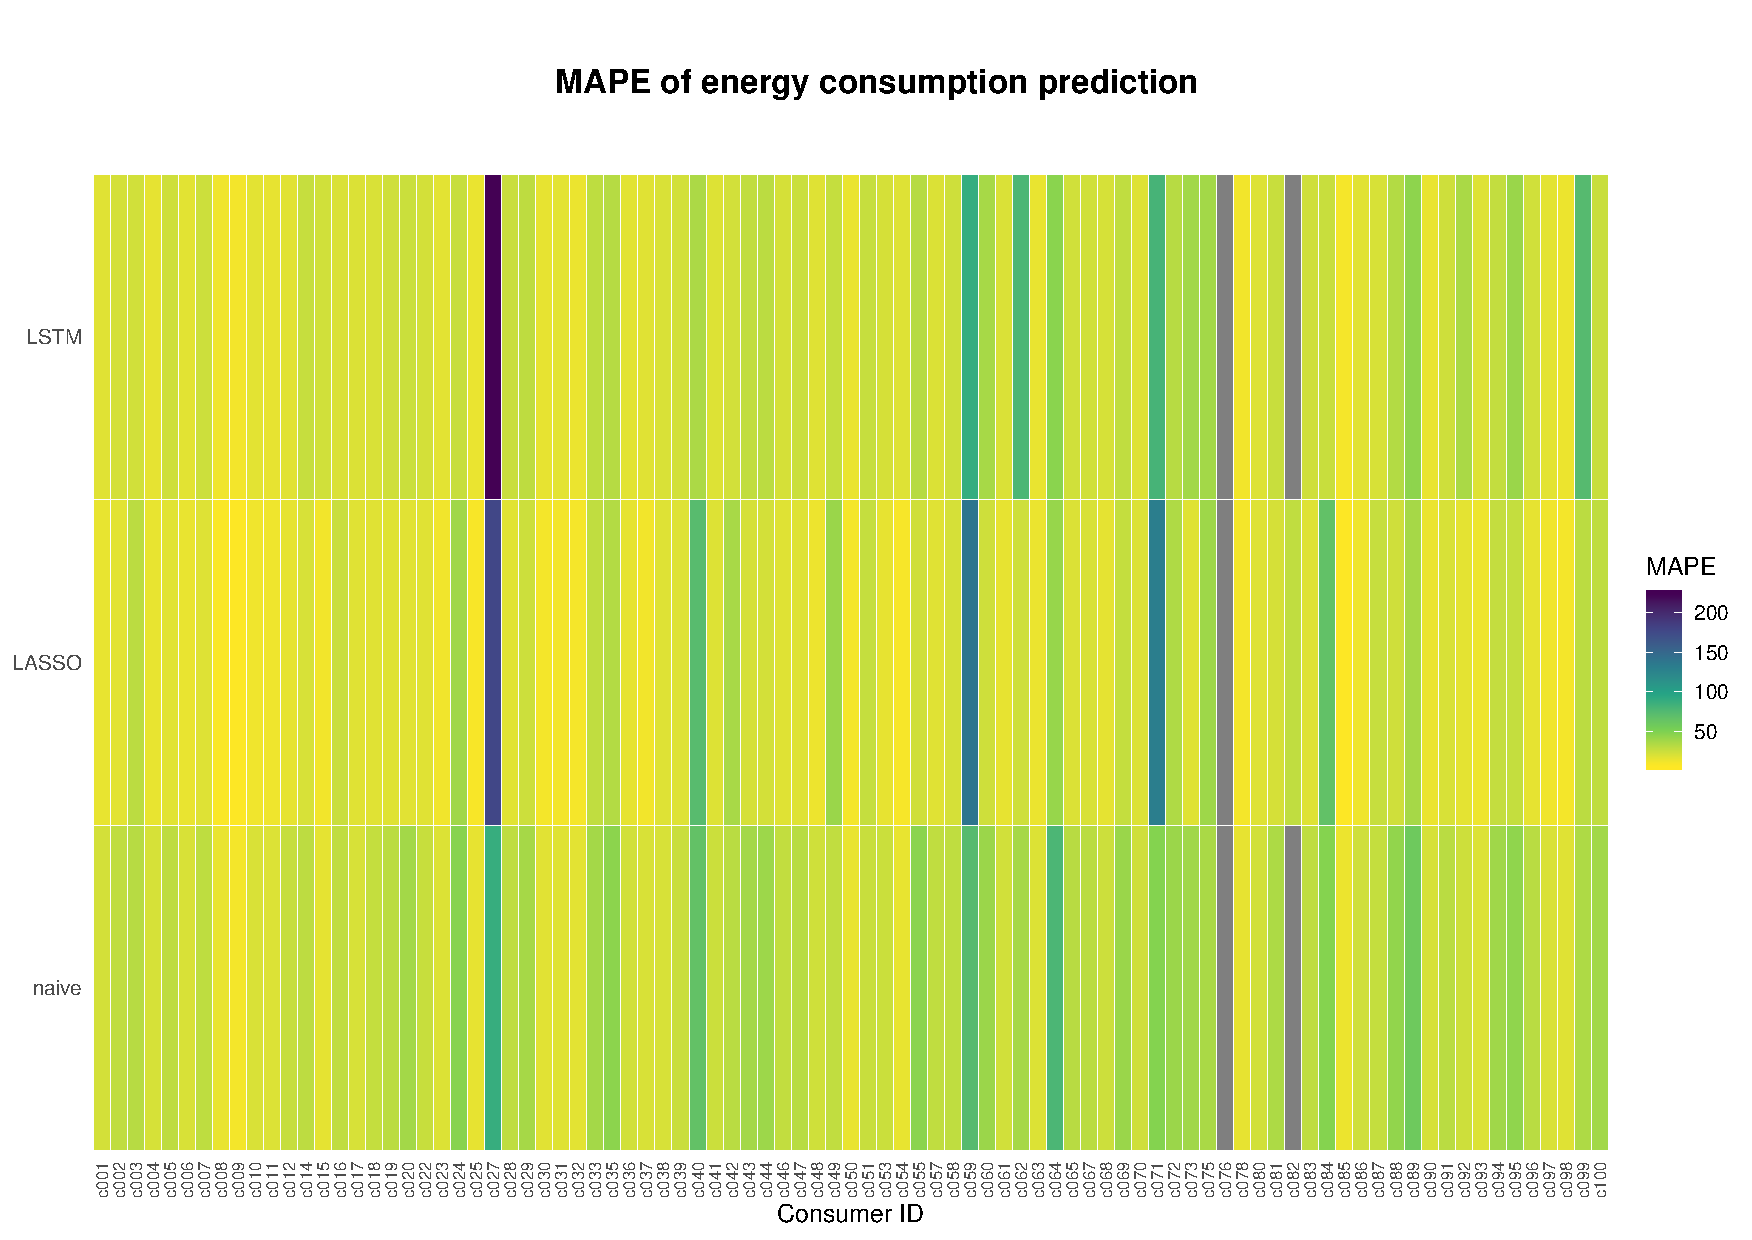
\includegraphics[width=\textwidth]{thesis/graphs/evaluation/c_heatmap_MAPE.pdf}
 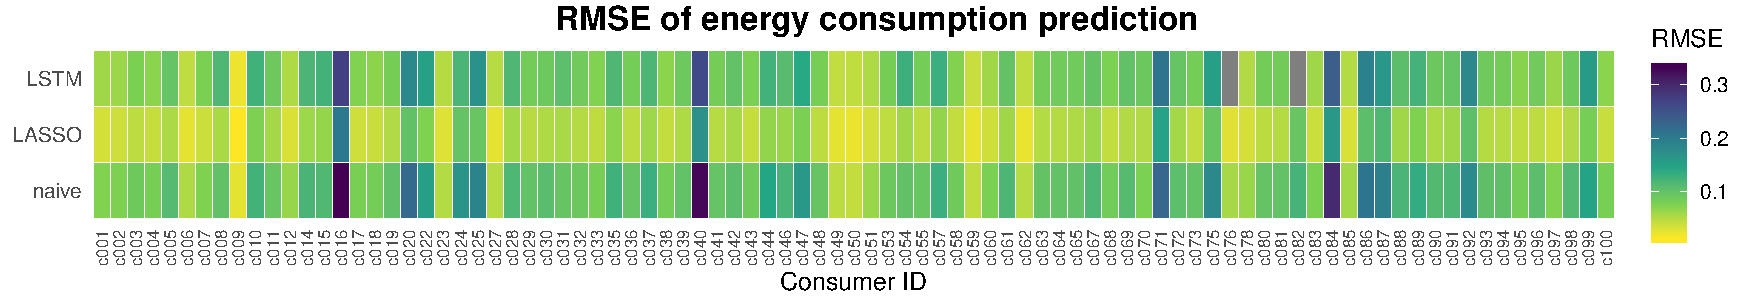
\includegraphics[width=\textwidth]{thesis/graphs/evaluation/c_heatmap_RMSE.pdf}
 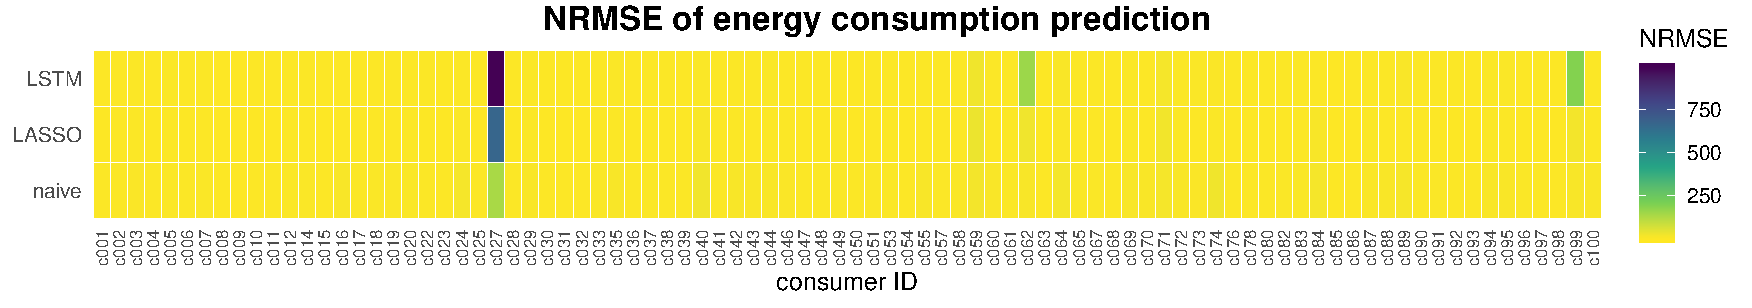
\includegraphics[width=\textwidth]{thesis/graphs/evaluation/c_heatmap_NRMSE.pdf}
 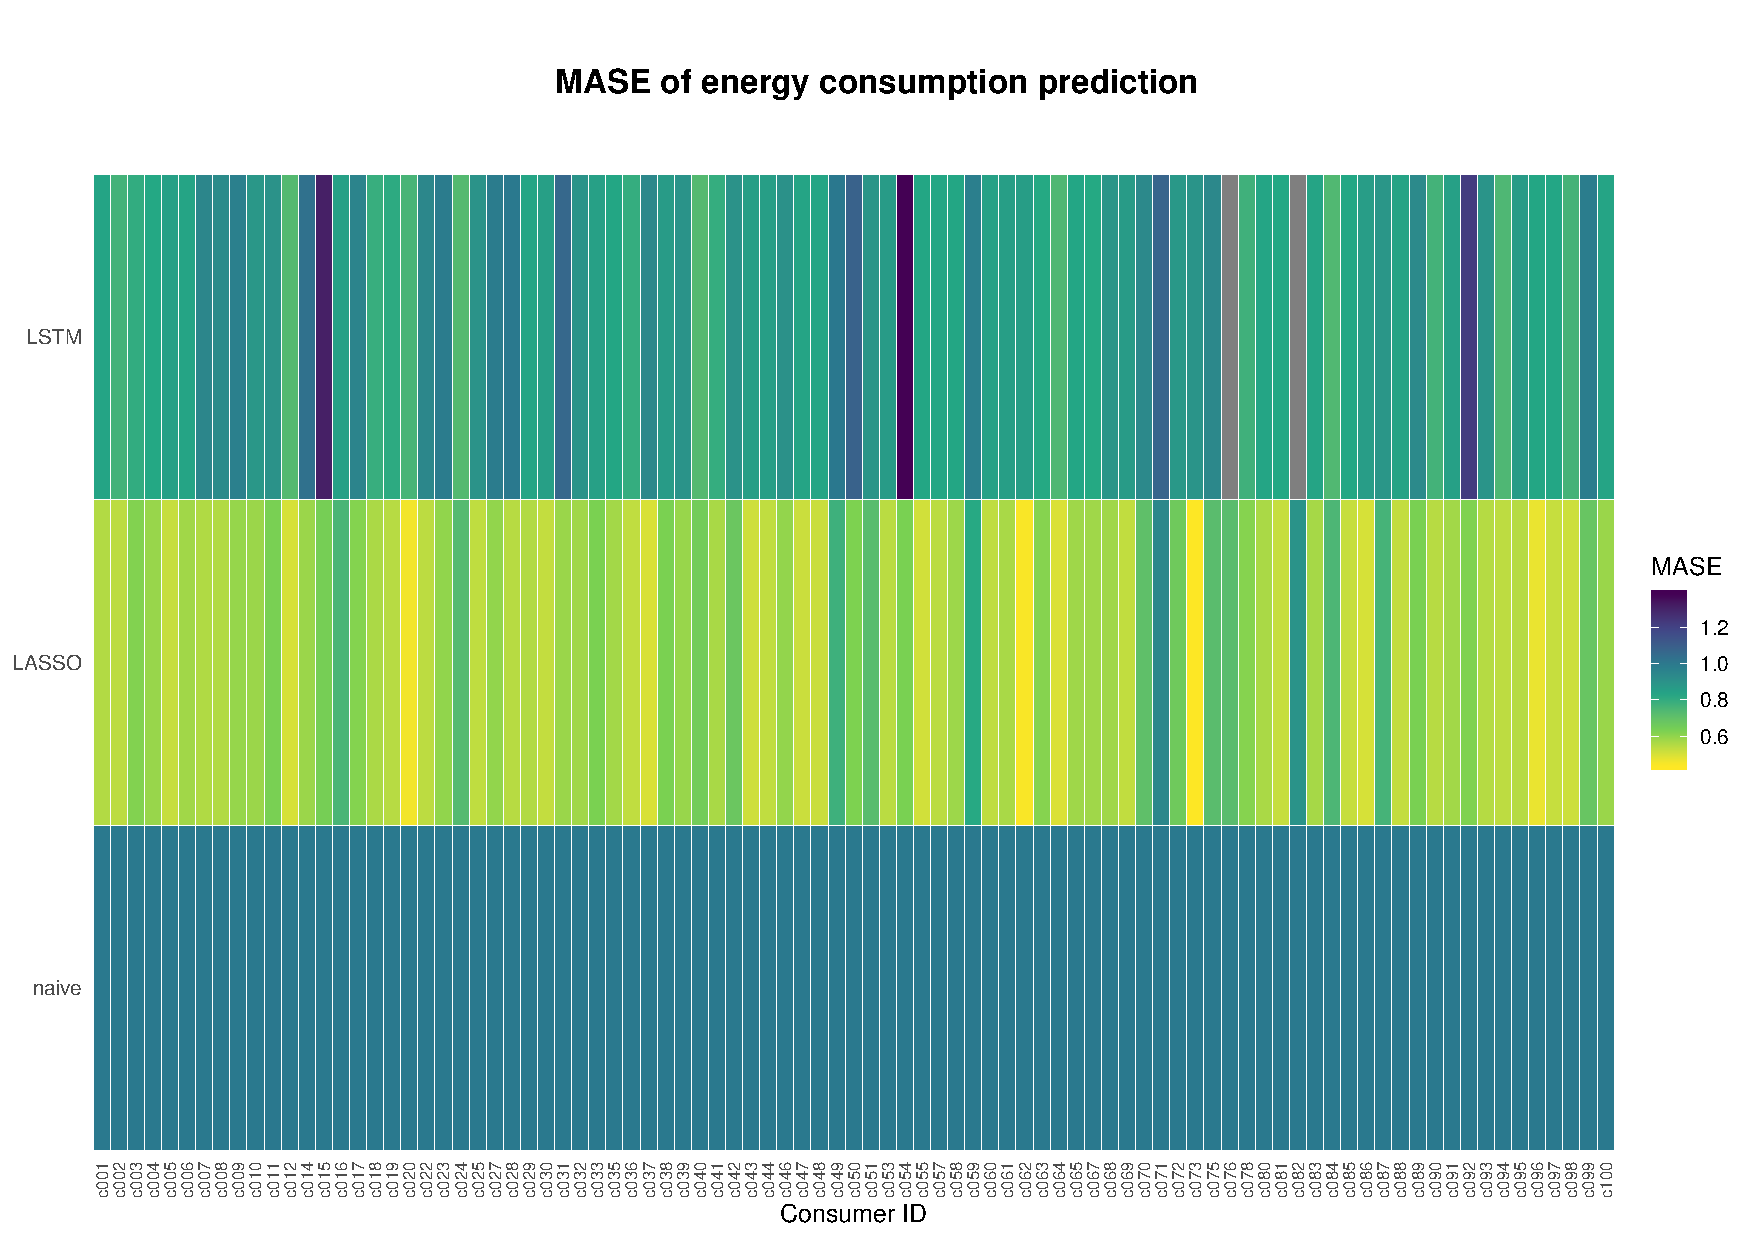
\includegraphics[width=\textwidth]{thesis/graphs/evaluation/c_heatmap_MASE.pdf}
\caption[Heatmaps of error measures for prediction of consumption values]{Heatmap of MAE, MAPE, RMSE, NRMSE, and MASE scores for the prediction of consumption values per consumer data set. \quantnet\href{https://github.com/QuantLet/BLEM/tree/master/BLEMevaluateEnergyPreds}{BLEMevaluateEnergyPreds}}
\label{Fig:heatmaps}
\end{figure}
%
 
Based on this insight, it seemed reasonable to reevaluate the average performance of the prediction methods across all consumer data sets using the median instead of the mean. Calculating the median error measures for all predictions on the consumer data sets eliminates the distortion by outliers. Thus, Table~\ref{Tab:median_errormeasures} shows the same error measures as Table~\ref{Tab:avg_errormeasures} but uses the median instead of the mean to summarize the models performance across all consumer data sets. This shows the LASSO model performed best overall with the lowest median MAE, RMSE, MAPE, NRMSE, and MASE scores. With a median MAPE across the 88 consumer datasets of 17.38~\%, it achieved an even better score in the present research than in the implementation of \citet{Li:2017}, who achieved a score of 20.06~\%.
%
\begingroup\catcode`"=9
\begin{table}[!hb]
{\footnotesize
    \csvreader[centered tabular=l|SSSSS,
    before reading=\sisetup{round-mode=places,round-precision=2,round-integer-to-decimal},
    filter not strcmp={\thecsvinputline}{1},
    table head=
    \hline\hline
     \multicolumn{1} {l}{\textbf{Model}} & \multicolumn{1} {c}{\textbf{MAE}} & \multicolumn{1} {c}{\textbf{RMSE}} & \multicolumn{1} {c}{\textbf{MAPE}} & \multicolumn{1} {c}{\textbf{NRMSE}} & \multicolumn{1} {c}{\textbf{MASE}}\\
    \hline,
    no head,
    separator=comma,
    respect all,
    late after line=\\,
    table foot=\hline \hline]
    {thesis/tables/median_errorMeasures.csv}{}%
    {\csvcolii & \csvcoliii & \csvcoliv & \csvcolv & \csvcolvi & \csvcolvii}}%
    \caption[Median of error measures for prediction on consumer data sets]{Median of error measures for the prediction of energy consumption across all 88 consumer data sets. \quantnet\href{https://github.com/QuantLet/BLEM/tree/master/BLEMevaluateEnergyPreds}{BLEMevaluateEnergyPreds}}
    \label{Tab:median_errormeasures}
\end{table}
\endgroup
%

The superior performance of the LASSO model is also clearly visible in Figure~\ref{Fig:boxplots_errormeasures}. Additionally noteworthy here are the differences in the IQR of the error measures between the prediction methods. Both, the LASSO as well as the LSTM model, have error measures with a smaller IQR across the consumer data sets than the benchmark model. Furthermore, even though the LASSO error measures consistently have the lowest median of all three prediction models, the IQR of the relative error measures MAPE and NRMSE is very similar between LASSO and LSTM.
%
\begin{figure}
    \centering
    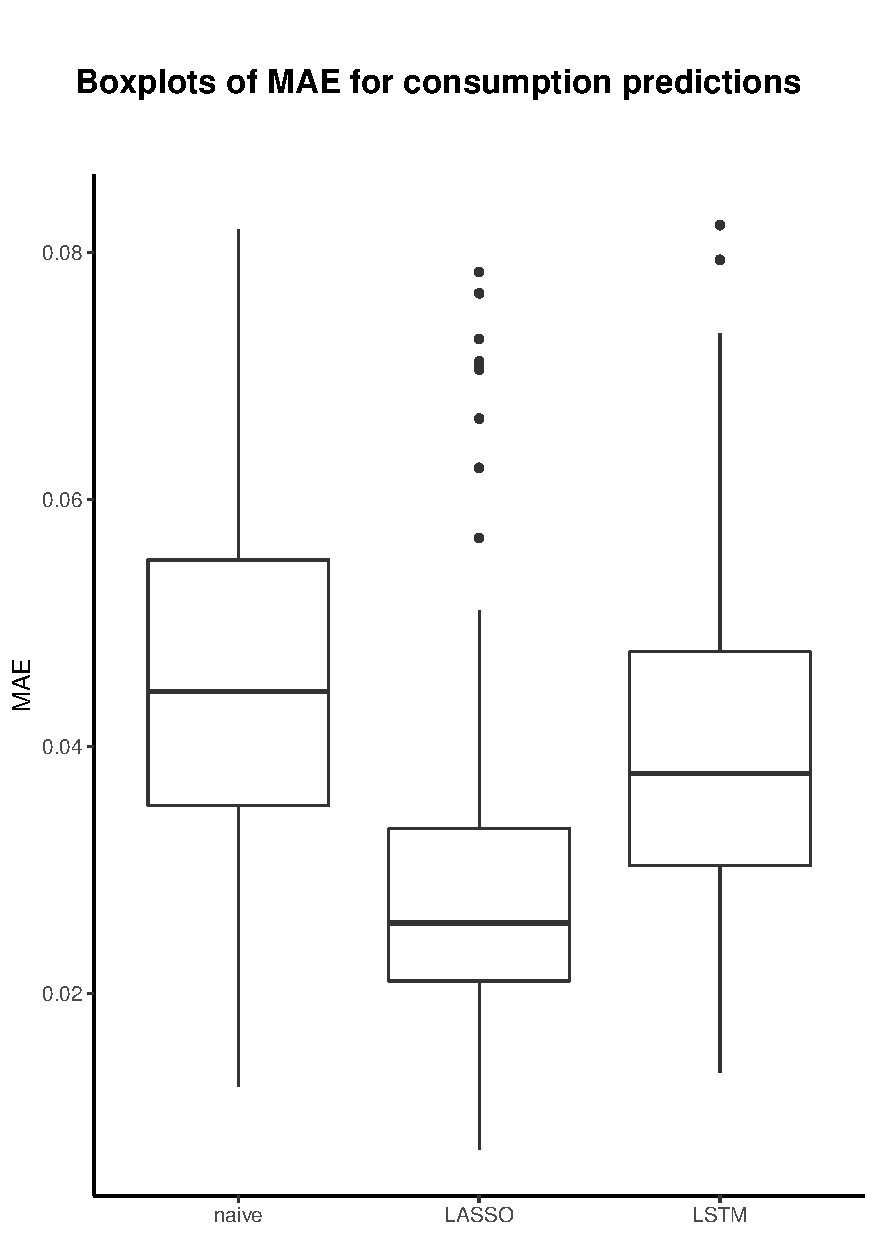
\includegraphics[width=.5\textwidth-5pt]{thesis/graphs/evaluation/c_boxplot_MAE.pdf}
    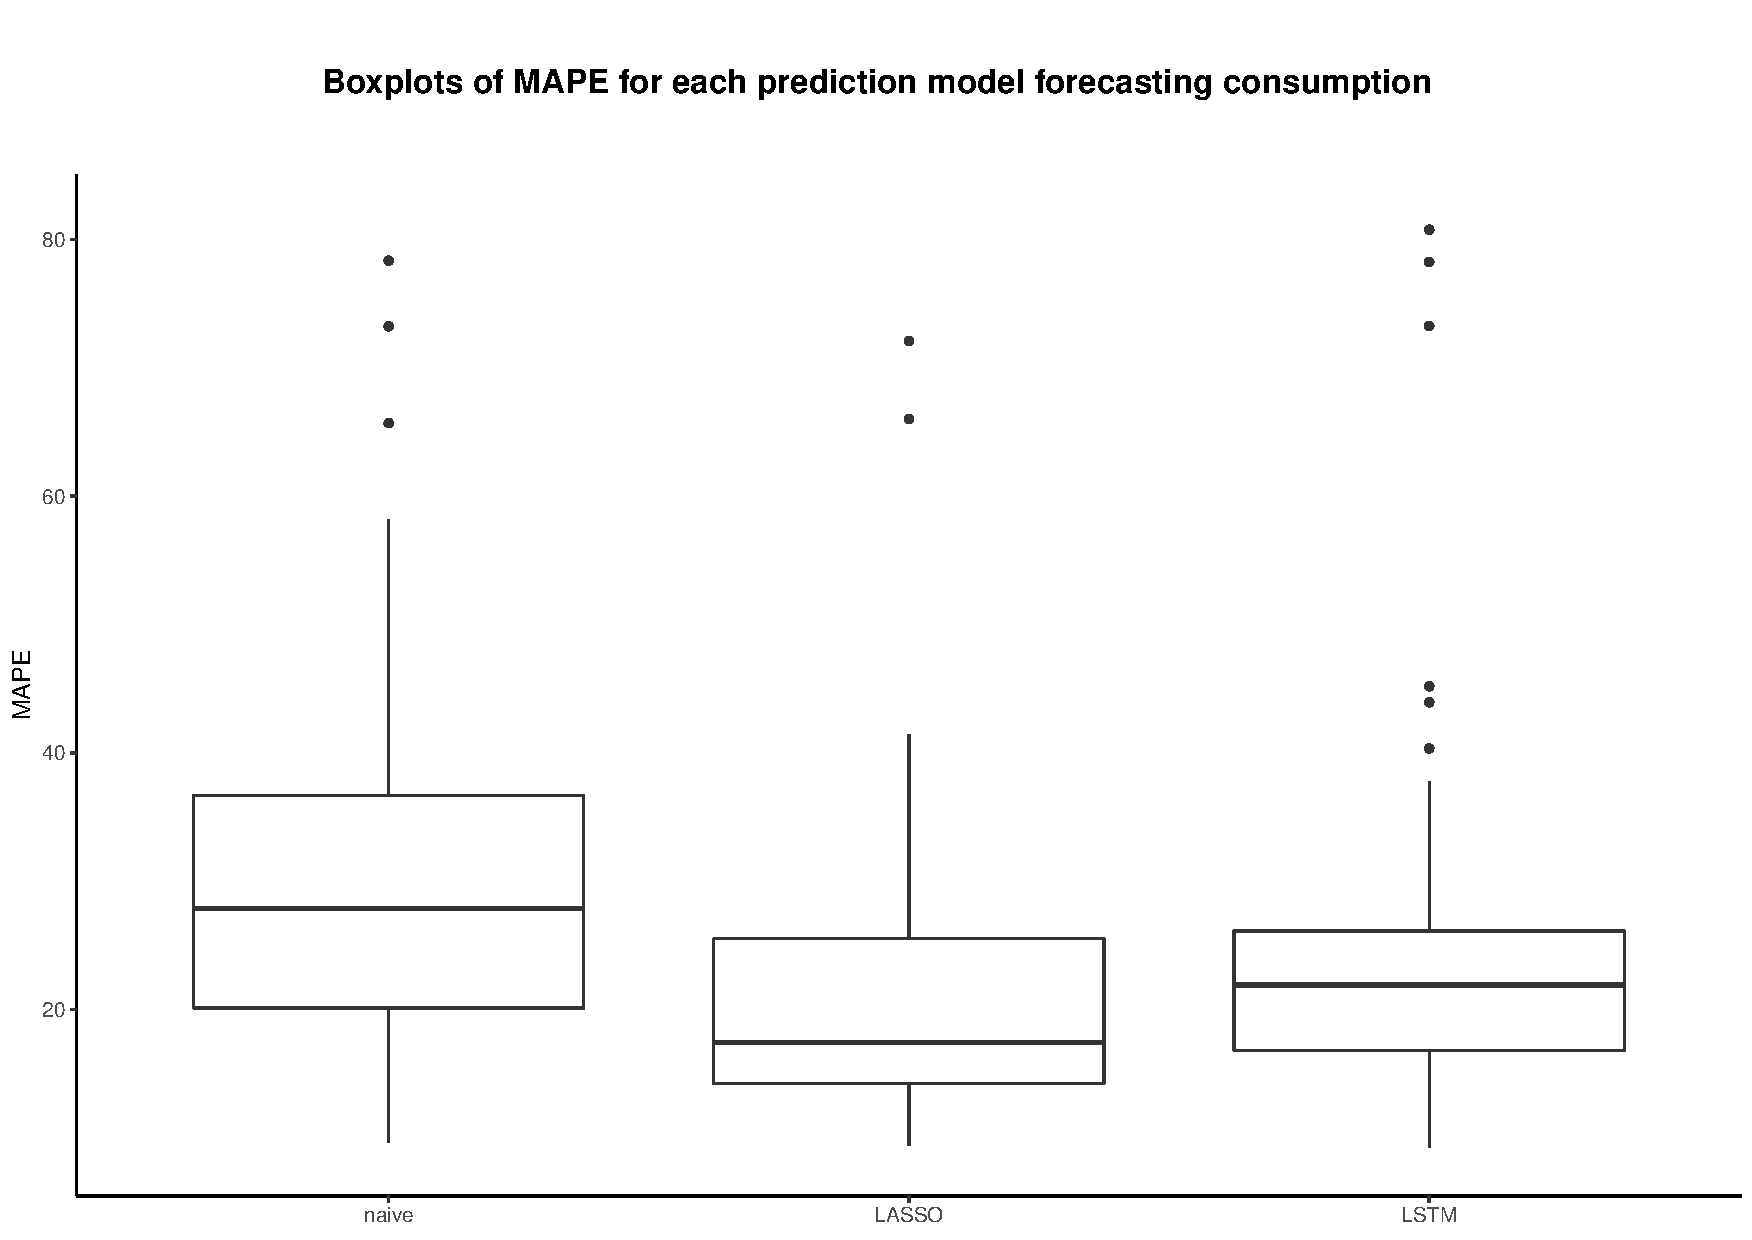
\includegraphics[width=.5\textwidth-5pt]{thesis/graphs/evaluation/c_boxplot_MAPE.pdf} \\
    
    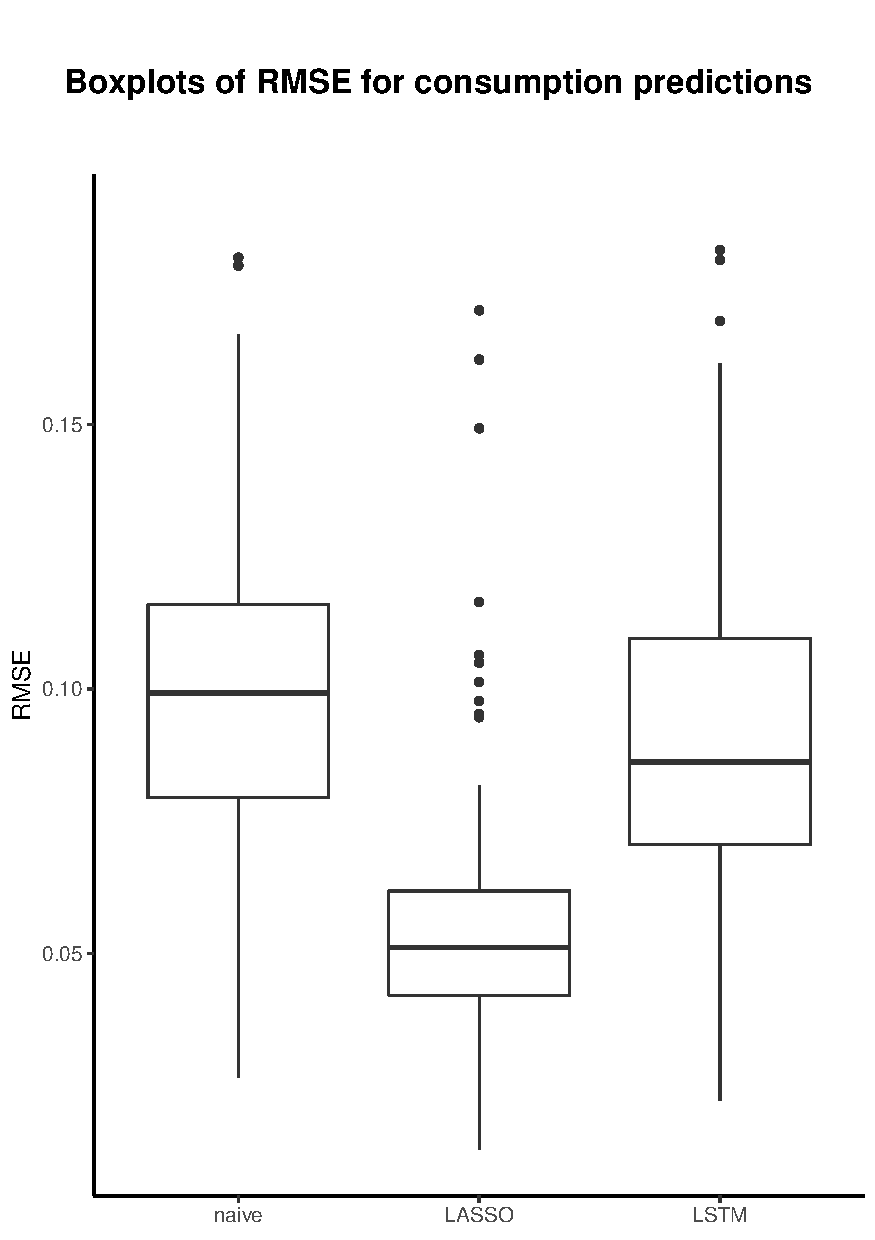
\includegraphics[width=.5\textwidth-5pt]{thesis/graphs/evaluation/c_boxplot_RMSE.pdf}
    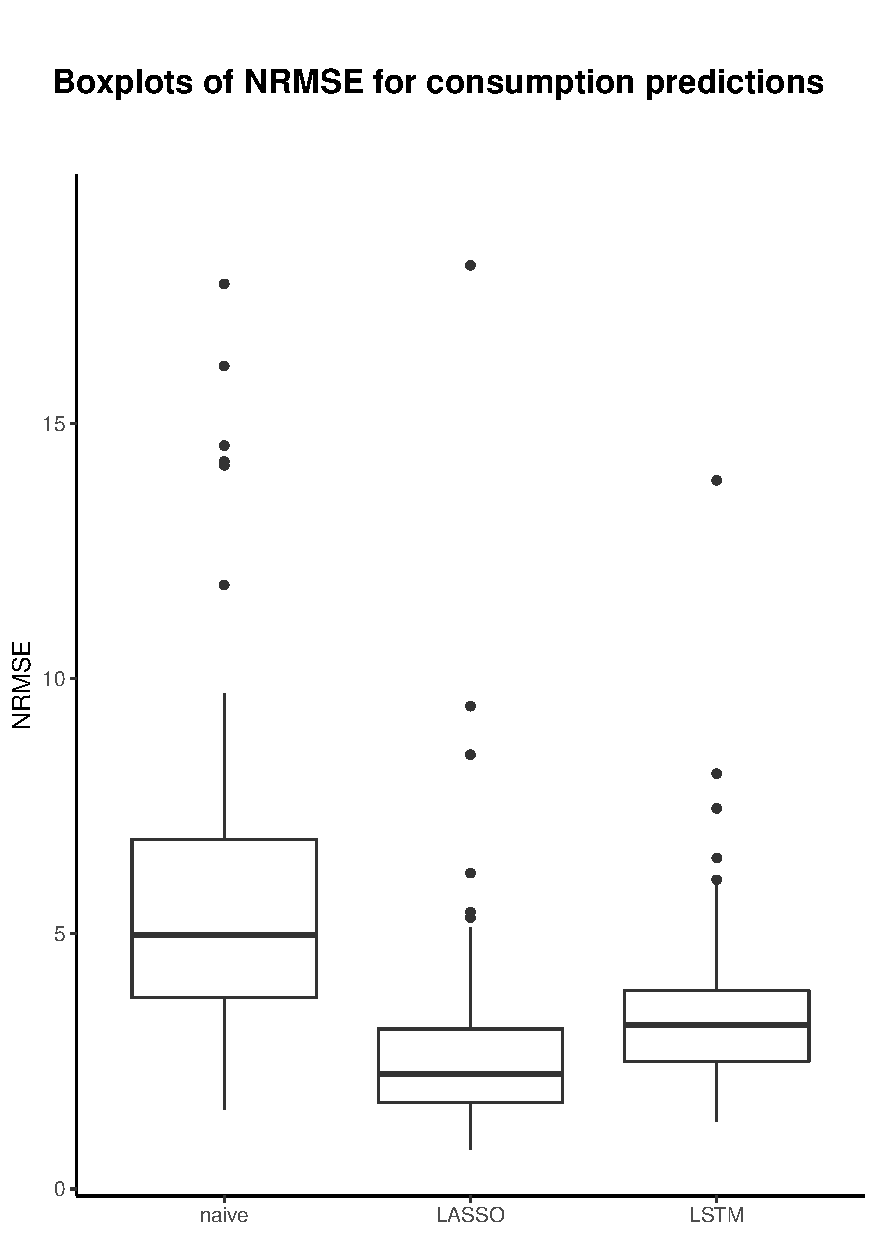
\includegraphics[width=.5\textwidth-5pt]{thesis/graphs/evaluation/c_boxplot_NRMSE.pdf} \\
    \caption[Boxplots of error measures for prediction of consumption values]{Boxplots of MAE, MAPE, RMSE, and NRMSE scores across 88 consumer data sets for the three different prediction models (the upper 3~\%-quantile of the error measures is cut off for better readability). \quantnet\href{https://github.com/QuantLet/BLEM/tree/master/BLEMevaluateEnergyPreds}{BLEMevaluateEnergyPreds}}
    \label{Fig:boxplots_errormeasures}
\end{figure}
%

\newpage
Interestingly, there are some consumer data sets which exhibit apparently much harder to predict consumption patterns than the other data sets. This is exemplified by the outliers of the MAPE and NRMSE boxplots, and also, by the heatmaps displayed in Figure~\ref{Fig:heatmaps}. Unfortunately, the heatmaps of the relative error measures MAPE and NRMSE are dominated by the very high values for consumer 027. An alternative way to calculate those error measures according to \citet{Hyndman:2006} to avoid very skewed NRMSE or MAPE distribution in the presence of values close to zero is to use the median instead of the mean error. Thus, the mean absolute percentage error becomes the median absolute percentage error (MdAPE) and the normalized root mean squared error becomes the normalized root median squared error (NRMdSE). Taking consumer 027 as an example, the difference becomes clear: The normalized root mean squared error is $\text{NRMSE}_{c027}=2383.46$, while the normalized root \emph{median} squared error is only $\text{NRMdSE}_{c027}=33.43$ (which is still comparatively high). The same holds true for MAPE and MdAPE\footnote{The average MdAPE and NRMdSE across all consumer data sets in comparison to MAPE and NRMSE are presented in Appendix~\hyperlink{AppB2:Tables:avg_errM_wMedian}{B2}.}. Accordingly, the heatmaps for MdAPE and NRMdSE are shown in Figure~\ref{Fig:heatmaps_median}. They confirm that there is a wide variation in the performance of the same prediction methods on the same kind of data but from different households. Therefore one can conclude, that apparently, there is no ``one-size-fits-all'' approach for households' very short-term energy consumption forecasting.

%
\begin{figure}[ht]
 \centering
 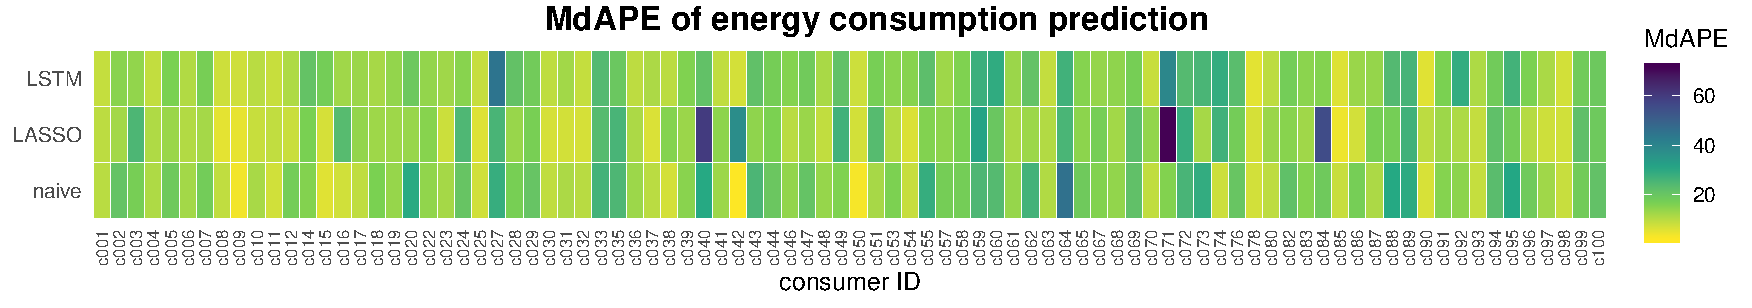
\includegraphics[width=\textwidth]{thesis/graphs/evaluation/c_heatmap_MdAPE.pdf}
 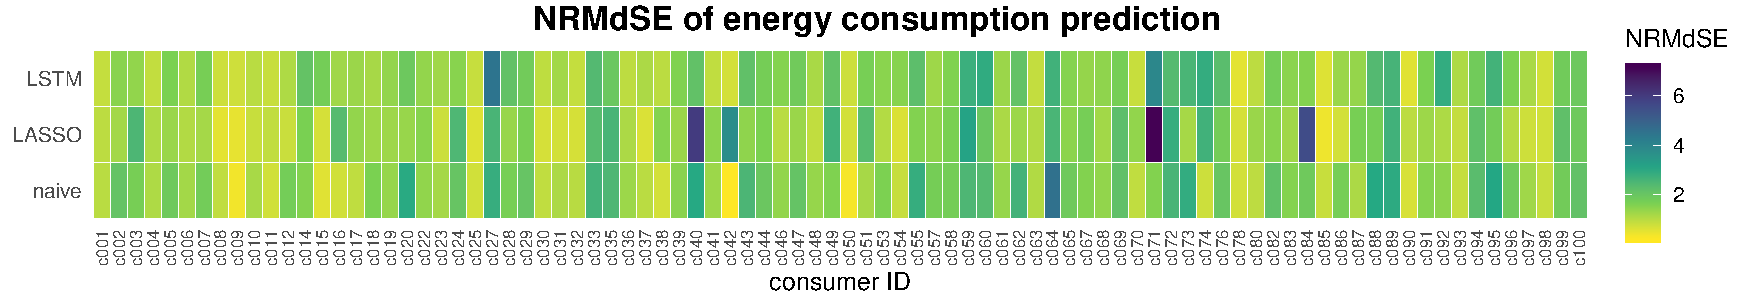
\includegraphics[width=\textwidth]{thesis/graphs/evaluation/c_heatmap_NRMdSE.pdf}
\caption[Heatmaps of MdAPE and NRMdSE for consumption values]{Heatmap of MdAPE and NRMdSE scores for the prediction of consumption values per consumer data set. \quantnet\href{https://github.com/QuantLet/BLEM/tree/master/BLEMevaluateEnergyPreds}{BLEMevaluateEnergyPreds}}
\label{Fig:heatmaps_median}
\end{figure}
%

Nevertheless, it is obvious that the LASSO model performed best overall. Hence, the predictions on the last quarter of the data produced by the fitted LASSO model for each consumer data set will be used for the evaluation of the following market simulation.



%%%%%%%%%%%
\subsubsection{Production data}

Also for the production data, the performance of the prediction models was tested on a quarter of the production time series. That is, the prediction models were fitted on the production values from 01.01.2017~00:00 to 30.09.2017~00:00 which is equivalent to 131,040 data points per data set. For all 12 prosumer data sets, the models were fitted separately resulting in as many distinct LASSO and LSTM prediction models. The fitted models were then used to make energy production predictions in 15-minutes intervals for each household individually on the data from 01.10.2017~00:00 to 01.01.2018~00:00. This equates to 8,836 predicted values per data set per prediction method.

Figure~\ref{Fig:glimpse_predprod} exemplary shows the true and predicted production values of prosumer 024 on December 23, 2017. The na\"ive benchmark model just follows the true production shifted by one time step (i.e., 15 minutes). As in the consumption predictions, this fits the true values generally good, as long as there are no sudden spikes in the household's energy production. Spikes or sudden drops in energy production -- as in this example one occurred in the 15 minutes before 06:00 a.m.~-- necessarily lead to a prediction with high error of the na\"ive predictor. In such situations, the LASSO model seems more accurate. Even though, it underestimates the spike in energy production in this example, it does not lag behind as much as the na\"ive predictor and, generally, has the ability to anticipate movements. The LSTM-based predictions, on the contrary, fit even worse than the na\"ive predictor in this example. They almost do not at all follow small movements in the energy production time series and lag behind the true values similarly to the na\"ive predictor. Also, the LSTM model constantly overestimates in periods of zero production and does not follow the upward spike in energy production present in this exemplary snippet of the data.
%
\begin{figure}[htbp]
    \centering
    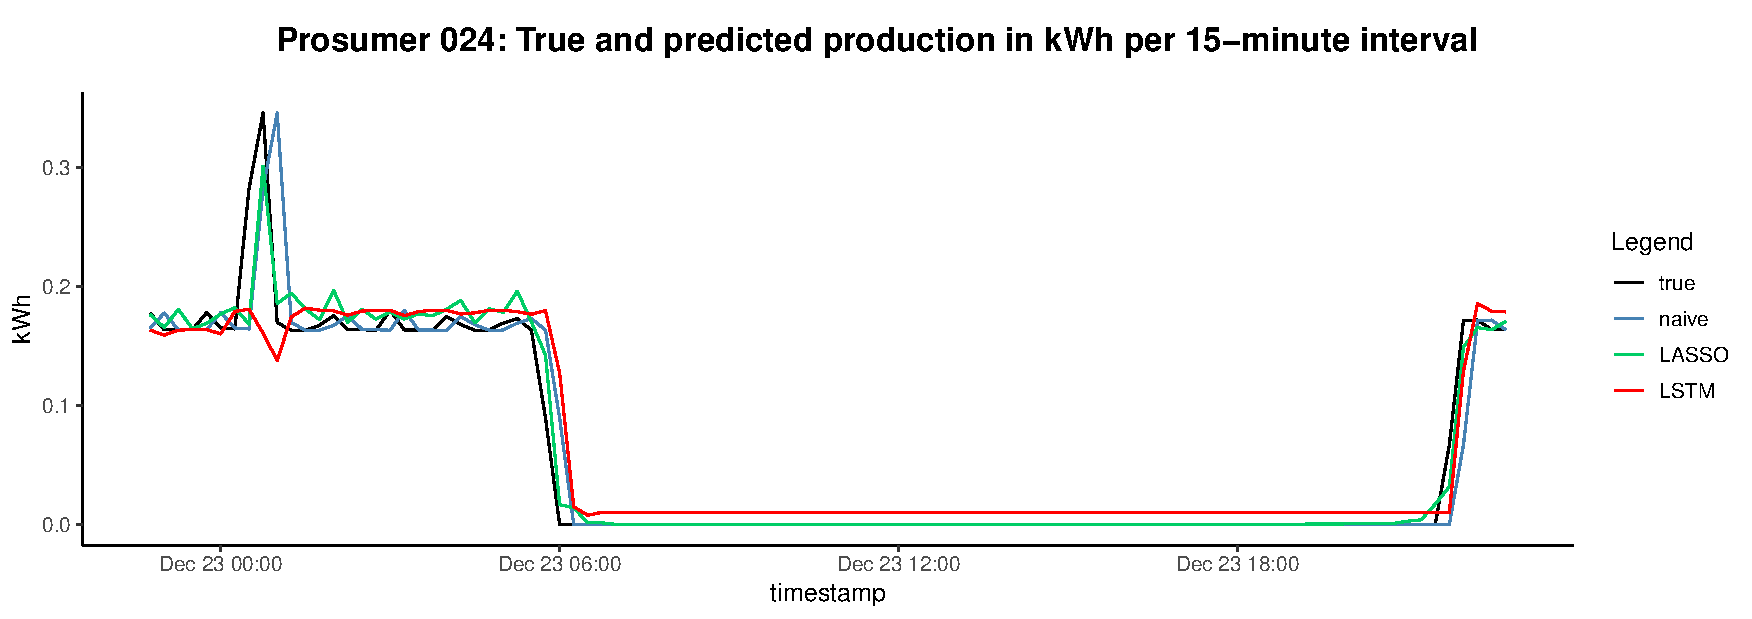
\includegraphics[width=\textwidth]{thesis/graphs/evaluation/p024_pred_prod.pdf}
    \caption[Exemplary 24 hours of true and predicted production values]{Exemplary 24 hours of true and predicted production values of prosumer 024. \quantnet\href{https://github.com/QuantLet/BLEM/tree/master/BLEMplotEnergyPreds}{BLEMplotEnergyPreds}}
    \label{Fig:glimpse_predprod}
\end{figure}
%

Analyzing the over- and underestimation errors of each prediction method on each producer data set shows the extreme tendency of the LSTM model to underestimate the production values (see Figure~\ref{Fig:overunderestimation_p}).
%
\begin{figure}[!h]
    \centering
    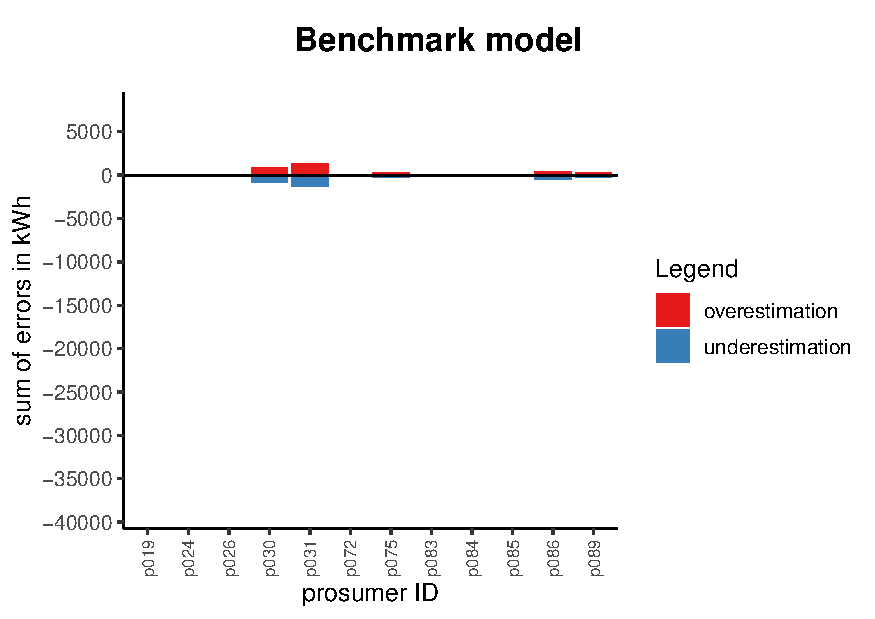
\includegraphics[width=.5\textwidth]{thesis/graphs/evaluation/p_barplot_naive_overunderestimation.pdf}\\\vspace{.6cm}
    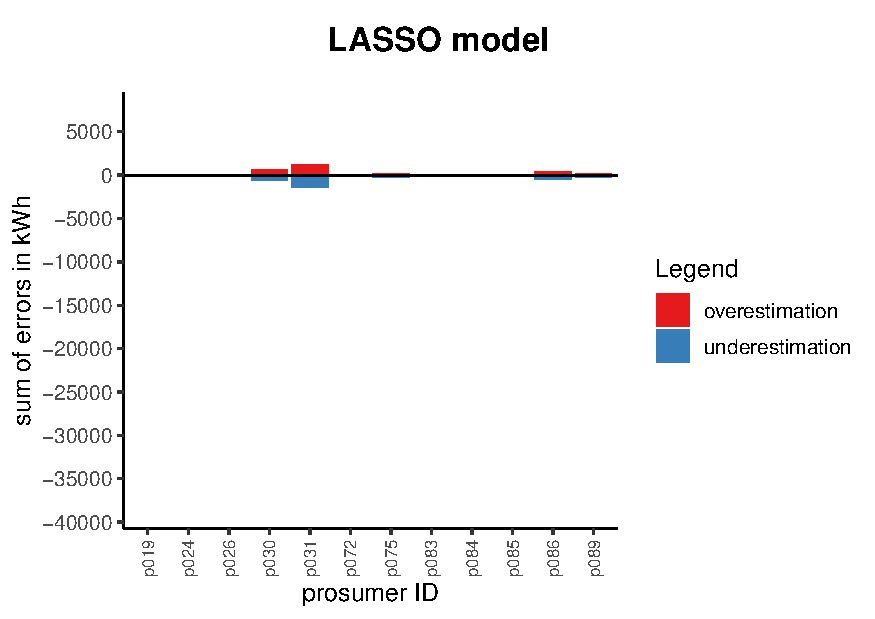
\includegraphics[width=.5\textwidth]{thesis/graphs/evaluation/p_barplot_LASSO_overunderestimation.pdf}\\\vspace{.6cm}
    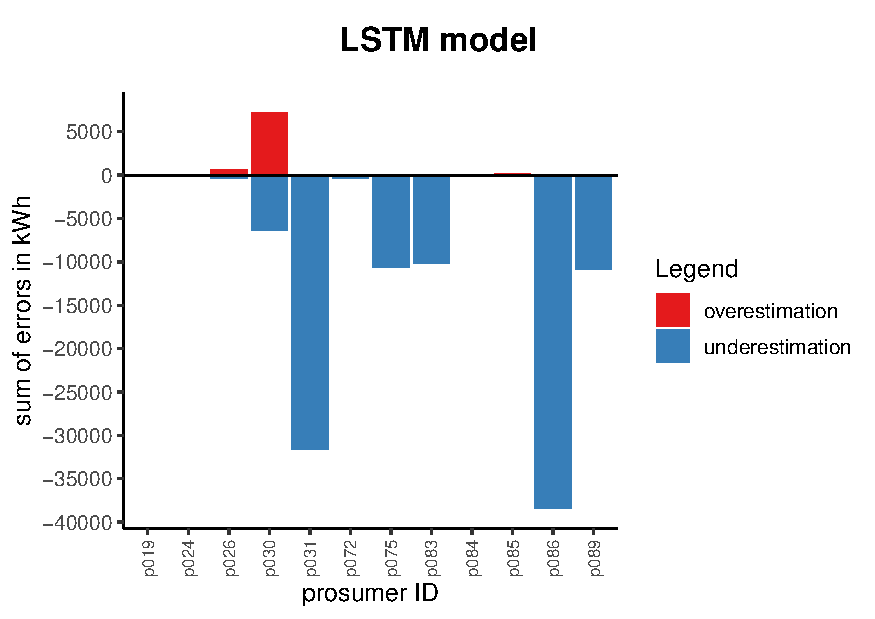
\includegraphics[width=.5\textwidth]{thesis/graphs/evaluation/p_barplot_LSTM_overunderestimation.pdf}
    \caption[Sum of total over- and underestimation errors per prosumer data set]{Sum of total over- and underestimation errors of energy production per prosumer data set and prediction model. \quantnet\href{https://github.com/QuantLet/BLEM/tree/master/BLEMplotPredErrors}{BLEMplotPredErrors}}
    \label{Fig:overunderestimation_p}
\end{figure}
%

The LSTM's sum of underestimation errors is substantially larger for six out of twelve prosumer data sets and the sum of overestimation is substantially larger for one data set compared to the LASSO and benchmark model. This already indicates a much worse performance of LSTM than LASSO or the na\"ive predictor on the production data.

The first impression is confirmed by the average of the error measures across the 12 prosumer data sets shown in Table~\ref{Tab:avg_errormeasures_p}. The LSTM model on average performs much worse than the LASSO and the benchmark model according to MAE, RMSE, and MASE. Computing the median across the 12 prosumer data sets gives the same qualitative results, although the performance differences are not as extreme (see Appendix~\hyperlink{AppB3:Tables:medain_errM_prod}{B3}). MAPE and NRMSE cannot be computed as all production time series contain zero values\footnote{As can be seen in Equation~\ref{Eq:MAPE} and Equation~\ref{Eq:NRMSE}, MAPE and NRMSE are not defined if the true value $x_t$ equals zero which is why they cannot be computed for the predictions on production data.}.
%
\begingroup\catcode`"=9
\begin{table}[ht]
{\footnotesize
    \csvreader[centered tabular=l|SSS,
    before reading=\sisetup{round-mode=places,round-precision=2,round-integer-to-decimal},
    filter not strcmp={\thecsvinputline}{1},
    table head=
    \hline\hline
     \multicolumn{1} {l}{\textbf{Model}} & \multicolumn{1} {c}{\textbf{MAE}} & \multicolumn{1} {c}{\textbf{RMSE}} & \multicolumn{1} {c}{\textbf{MASE}}\\
    \hline,
    no head,
    separator=comma,
    respect all,
    late after line=\\,
    table foot=\hline \hline]
    {thesis/tables/avg_errorMeasures_p.csv}{}%
    {\csvcolii & \csvcoliii & \csvcoliv & \csvcolv}}%
    \caption[Mean of error measures for prediction on prosumer data sets]{Mean of error measures for the prediction of energy production across all 12 prosumer data sets. \quantnet\href{https://github.com/QuantLet/BLEM/tree/master/BLEMevaluateEnergyPreds}{BLEMevaluateEnergyPreds}}
    \label{Tab:avg_errormeasures_p}
\end{table}
\endgroup
%

Overall, it becomes clear that the chosen prediction methods do not forecast energy production of the given prosumer data sets very well. According to the average MASE, the LASSO model is just as good as the benchmark, while the LSTM model performs much worse. A detailed comparison of the error measures for each prosumer data set as heatmap is shown in Appendix~\hyperlink{AppA5:Figures:heatmaps_p}{A5}. Due to the unsatisfying performance of the prediction methods on the production data, the predicted production values were not used in the market simulation. This means, the effect of prediction errors on market outcomes was only evaluated using the predictions of consumption values. The production values, on the contrary, were always assumed to be known in advance.

% In the case of the LSTM model, this may be due to the hyperparameter tuning being performed on a consumer data set. Moreover, the production data contains much more jumps and discontinuities than the consumption data which aggravates the prediction task.


%%%%%%%%%%%%%%%%%%%%%%%%%%%%%
%%%   Market simulation   %%%
%%%%%%%%%%%%%%%%%%%%%%%%%%%%%

\subsection{Evaluation of the market simulation}\label{Sec:Results;Subsec:Simulation}

The market simulation used the market mechanism implemented by \citet{Mengelkamp:2018a} in a smart contract to assess the impact of prediction errors on market outcomes. The data sets available for this comprised 88 consumers and 12 prosumers. To evaluate different supply scenarios, the market simulation was conducted three times with a varying number of prosumers included. The three scenarios consisted of a market simulation with balanced energy supply and demand, a simulation with severe oversupply and a simulation with severe undersupply. To avoid extreme and unusual market outcomes over the time period of the simulation, two prosumers (031 and 086) with high production levels, but long periods of no energy production in the simulation period were not included as energy suppliers in the market (see Appendix~\hyperlink{AppA7:Figures:producer_all}{A7}). The remaining prosumers were in- or excluded according to the desired supply scenario. That is, the undersupply scenario comprised prosumer 019, 024, 026, 072, 075, and 089, the balanced supply scenario additionally included prosumer 030, and the oversupply scenario additionally included prosumer 083 and 084.

%%%%%%%%%%%
\subsubsection{Market outcomes in different supply scenarios}

The difference between supply and demand for each trading period, the equilibrium price of each double auction, and the weighted average price -- termed LEM price -- is shown in Figure~\ref{Fig:marketoutcomes_true_balanced}. The LEM price is computed in each trading period as the average of the auctions equilibrium price and the energy utilities energy price (28.69 $\frac{\text{EURct}}{\text{kWh}}$) weighted by the amount of kWh traded for the respective price. Therefore, in any trading period with higher demand than supply, the LEM price will be greater or equal to the equilibrium price as the equilibrium price's upper limit is the utilities energy price of 28.69 $\frac{\text{EURct}}{\text{kWh}}$. All graphs depicting the market outcomes shown in this section are results of the market simulation with true consumption values. The equivalent graphs for the market simulation with energy consumption values predicted by a LASSO model are shown in Appendix~\hyperlink{AppA7:Figures:marketsimulation_pred}{A7}. As the graphs contain only over-/undersupply and market prices, they are not substantially different when simulating the market mechanism with predicted consumption values (as the prediction accuracy is reasonably good). Though, this is not the case for the energy cost that consumers have to bear, as is shown in the next section.

As can be seen, the equilibrium price shown in the middle panel of Figure~\ref{Fig:marketoutcomes_true_balanced} moves roughly synchronous to the over-/undersupply shown in the upper panel. As there is by tendency more undersupply in the balanced scenario (the red line in the upper panel indicates perfectly balanced supply and demand), the equilibrium price is in most trading periods close to its upper limit and the LEM price is almost always above the equilibrium price\footnote{Due to the fact that four of the relevant prosumer data sets are from producers with large capacities ($>$10 kWh per 15-minutes interval) which dominated the remaining prosumers' production capacity substantially (see also Appendix~\hyperlink{AppA7:Figures:producer_all}{A7}), it was not possible to construct a prosumer sample that better matched the market demand in the balanced supply scenario.}.
%
\begin{figure}[htp]
    \centering
    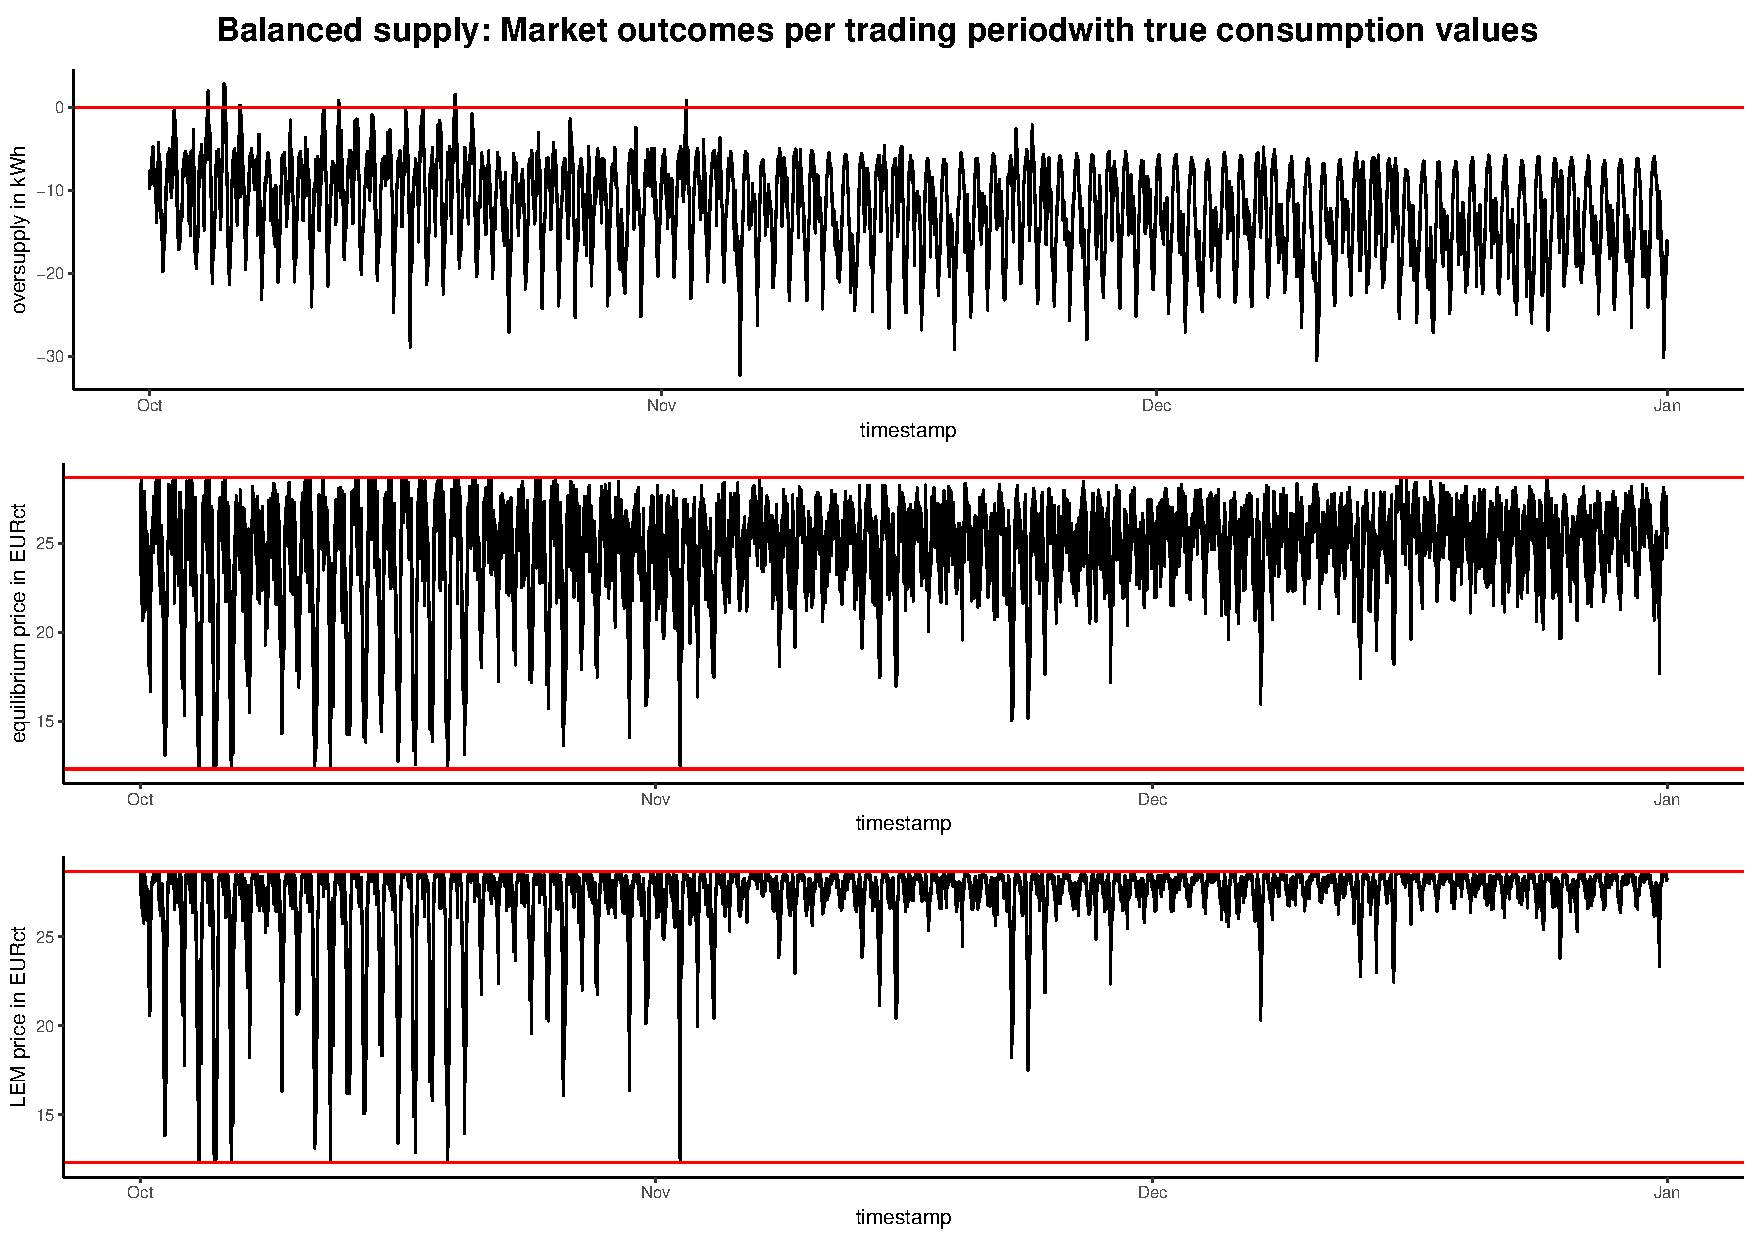
\includegraphics[width=\textwidth-1.1cm]{thesis/graphs/marketsimulation/marketoutcome_true_balanced.pdf}
    \caption[Market outcomes simulated with balanced supply and true values]{Market outcomes per trading period simulated with true values and a balanced supply scenario. \quantnet\href{https://github.com/QuantLet/BLEM/tree/master/BLEMmarketSimulation}{BLEMmarketSimulation}}
    \label{Fig:marketoutcomes_true_balanced}
\end{figure}
%

This is very much contrasted by the oversupply scenario shown in Figure~\ref{Fig:marketoutcomes_true_over}. Here, the prosumers' energy supply surpasses the consumers' energy demand in the majority of trading periods. Accordingly, the equilibrium price in each auction is close to the lower limit of the energy utility's feed-in tariff of 12.31 $\frac{\text{EURct}}{\text{kWh}}$. Still, trading periods with undersupply lead to visible spikes in the equilibrium price which are, as expected, even more pronounced in the LEM price. In all other periods, the equilibrium price equals the LEM price as all demand is served by the prosumers and there is no energy purchased from the grid.
%
\begin{figure}[htp]
    \centering
    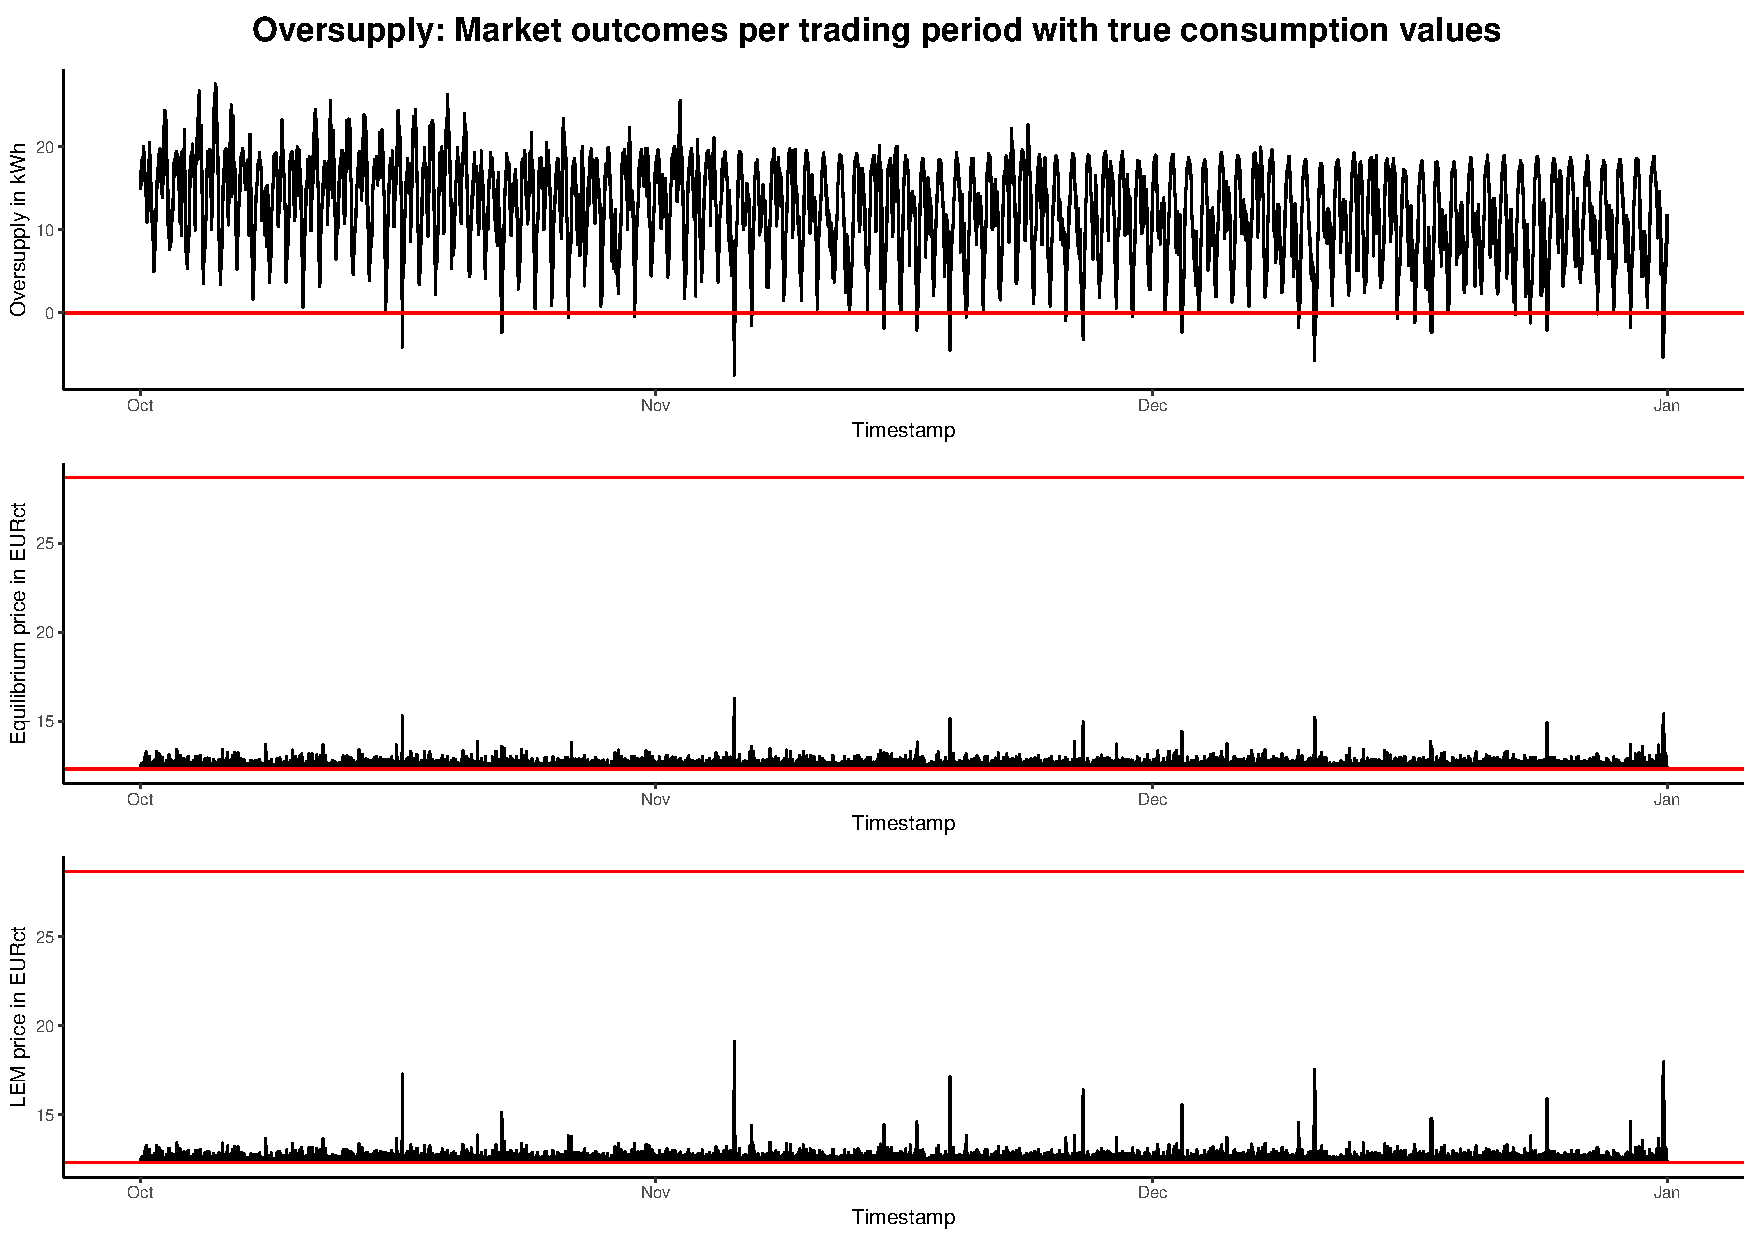
\includegraphics[width=\textwidth-1.1cm]{thesis/graphs/marketsimulation/marketoutcome_true_oversupply.pdf}
    \caption[Market outcomes simulated with oversupply and true values]{Market outcomes per trading period simulated with true values and an oversupply scenario. \quantnet\href{https://github.com/QuantLet/BLEM/tree/master/BLEMmarketSimulation}{BLEMmarketSimulation}}
    \label{Fig:marketoutcomes_true_over}
\end{figure}
%

Figure~\ref{Fig:marketoutcomes_true_under} shows the market simulation performed in a undersupply scenario. Here, as one would expect, the market outcomes are the opposite to the oversupply scenario. The equilibrium prices move in a band between 20 $\frac{\text{EURct}}{\text{kWh}}$ and the upper limit of 28.69 $\frac{\text{EURct}}{\text{kWh}}$. The LEM prices are even higher in each period as the deficit in supply has to be compensated by energy purchases from the grid. This means, the more severe the undersupply, the more energy has to be purchased from the grid, and the more the LEM price surpasses the equilibrium price.
%
\begin{figure}[htp]
    \centering
    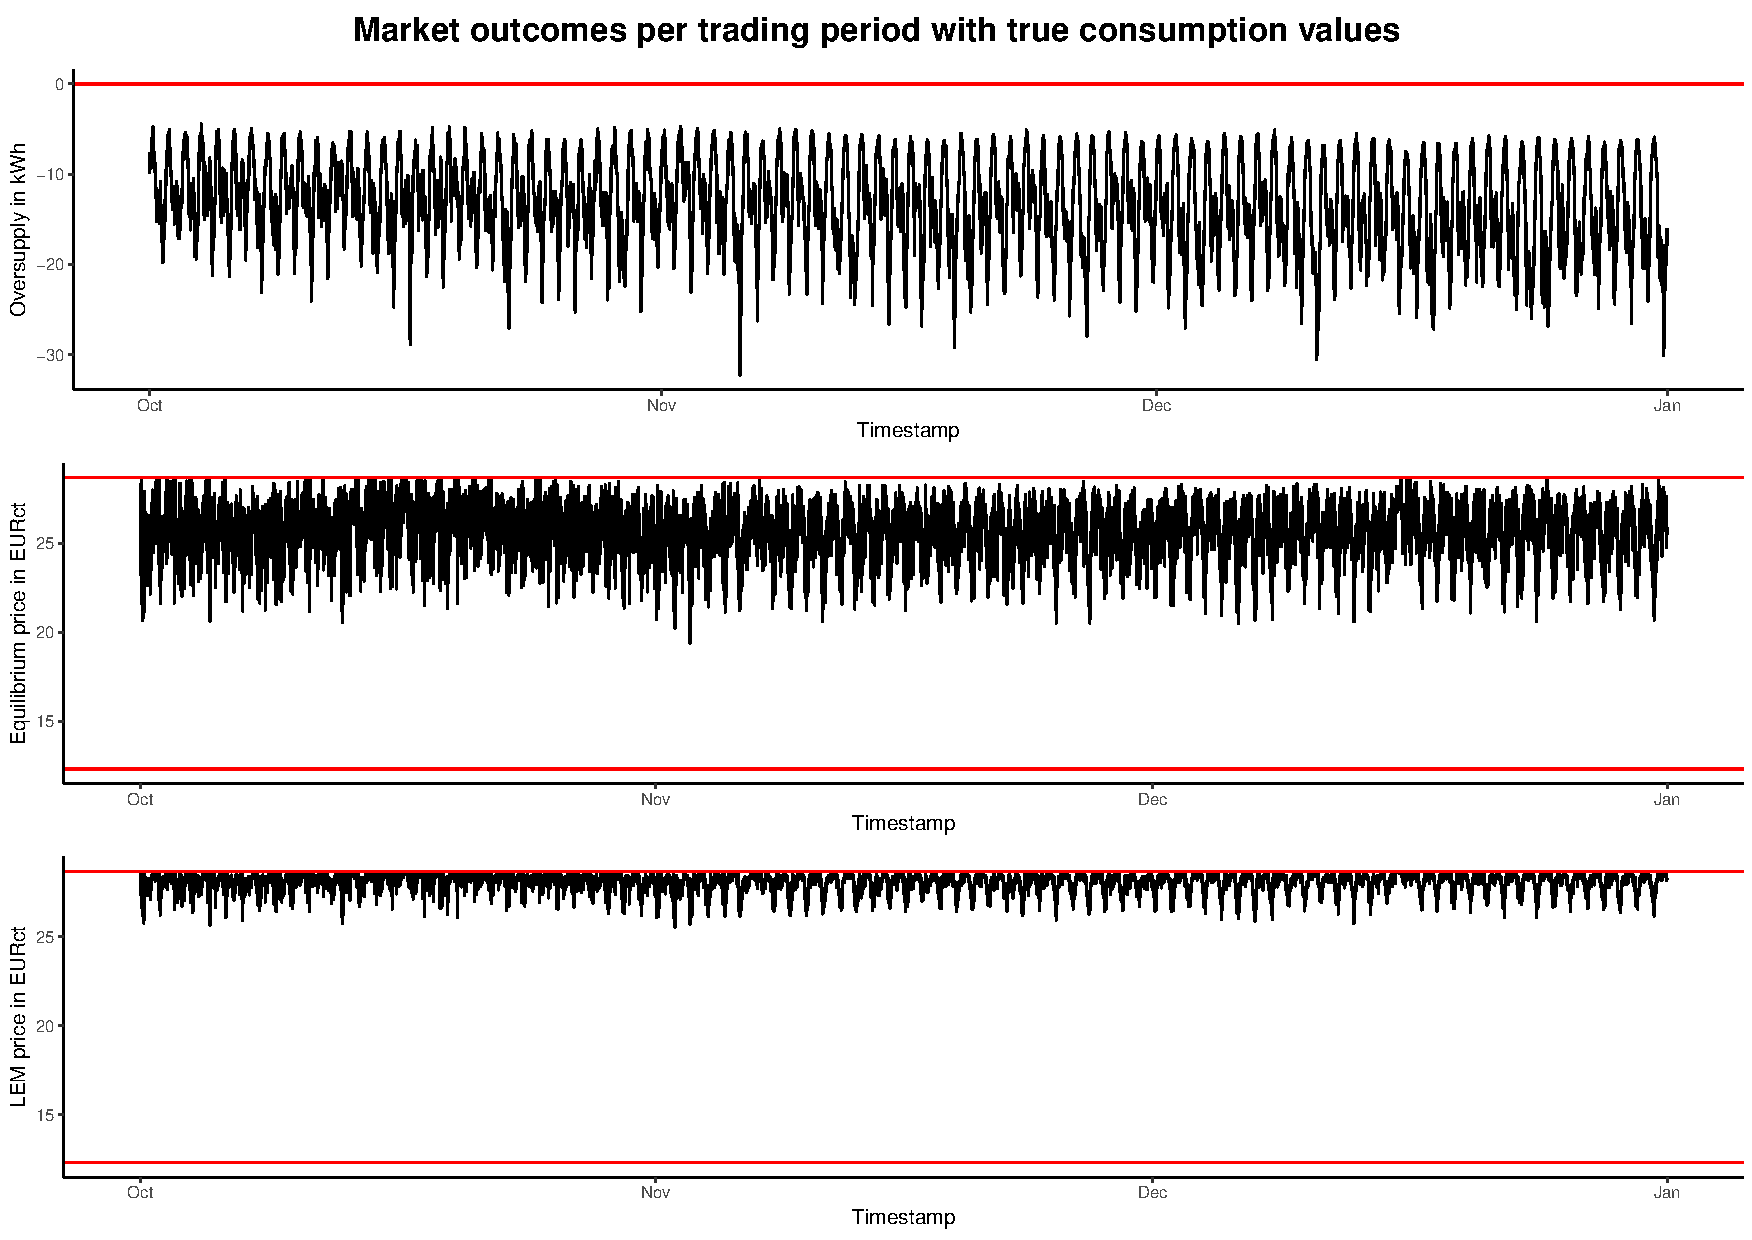
\includegraphics[width=\textwidth-1.1cm]{thesis/graphs/marketsimulation/marketoutcome_true_undersupply.pdf}
    \caption[Market outcomes simulated with undersupply and true values]{Market outcomes per trading period simulated with true values and an undersupply scenario. \quantnet\href{https://github.com/QuantLet/BLEM/tree/master/BLEMmarketSimulation}{BLEMmarketSimulation}}
    \label{Fig:marketoutcomes_true_under}
\end{figure}
%
\newpage
In summary, one can conclude that the market outcomes are the more favourable to consumers, the more locally produced energy is offered by prosumers. Assuming a closed double auction as market mechanism and zero-intelligence bidding behavior of market participants, oversupply reduces the LEM prices substantially leading to savings on the consumer side. On the other hand, prosumers will favor undersupply in the market as they profit from the high equilibrium prices while still being able to sell their surplus energy generation at the feed-in tariff without a loss compared to no LEM. Table~\ref{Tab:simulationresults} summarizes these results.


%%%%%%%%%%%
\subsubsection{Loss to consumers due to prediction errors}

To assess the adverse effect of prediction errors on the market outcomes, the LASSO-predicted energy consumption values per 15-minutes interval were used. The predictions of the model served as basis for the auction bids. After the true consumption in the respective trading period was observed, payments to settle over- or underestimation errors were made. That is, if a consumer bid with a higher amount than actually consumed, it still bought the full bid amount from the prosumers but had to sell the surplus to the energy utility over the grid at the feed-in tariff. On the other hand, if a consumer bid with a lower amount than actually consumed, it bought the bid amount from the prosumers but had to purchase the surplus energy consumption from the grid at the energy utility's tariff. Thus, prediction errors are costly as the consumer always has to clear the order at less favourable conditions than the equilibrium price provides.

Table~\ref{Tab:simulationresults} contrasts the results of the market simulation with true consumption values with the results of the market simulation with predicted values in three different supply scenarios.
%
\begingroup\catcode`"=9
\begin{table}[h]
{\footnotesize
    \csvreader[centered tabular=l|SSSSSS,
    before reading=\sisetup{round-mode=places,round-precision=2,round-integer-to-decimal},
     filter not strcmp={\thecsvinputline}{1},
     %filter expr={
      %test{\ifnumgreater{\thecsvinputline}{2}}},
    table head=
    \hline\hline
     \multirow{2}{2em}{\textbf{Mean}} & \multicolumn{2} {c}{\textbf{Balanced supply}} & \multicolumn{2} {c}{\textbf{Oversupply}} & \multicolumn{2} {c}{\textbf{Undersupply}}\\
     & \multicolumn{1} {c}{\textbf{true}} & \multicolumn{1} {c}{\textbf{predicted}} & \multicolumn{1} {c}{\textbf{true}} & \multicolumn{1} {c}{\textbf{predicted}} & \multicolumn{1} {c}{\textbf{true}} & \multicolumn{1} {c}{\textbf{predicted}}\\
    \hline,
    no head,
    separator=comma,
    respect all,
    late after line=\\,
    table foot=\hline \hline]
    {thesis/tables/average_outcomes.csv}{}%
    {\csvcolii & \csvcoliii & \csvcoliv & \csvcolv & \csvcolvi & \csvcolvii & \csvcolviii}}%
    \caption[Outcomes of market simulation for different supply scenarios]{Average results of the market simulation for three different supply scenarios. Prices are averaged across all trading periods. Revenues and costs for the whole simulation period are averaged across all prosumers and consumers respectively. \quantnet\href{https://github.com/QuantLet/BLEM/tree/master/BLEMevaluateMarketSim}{BLEMevaluateMarketSim}}
    \label{Tab:simulationresults}
\end{table}
\endgroup
%
\linebreak
The equilibrium and LEM prices almost do not differ within the three scenarios whether the true or predicted consumption values are used. However, the prices between the scenarios differ substantially as was already indicated by Figures~\ref{Fig:marketoutcomes_true_balanced}, \ref{Fig:marketoutcomes_true_over} and \ref{Fig:marketoutcomes_true_under}. Furthermore, the average total revenue over the three month simulation period of the prosumers is largely unaffected by the use of true or predicted consumption values. This is not surprising as the revenue is a function of the equilibrium price, which is apparently largely unaffected by whether true or predicted consumption values are used, and the electricity produced, which is obviously completely unaffected by whether true or predicted consumption values are used. This might be different if also predicted instead of true production values were used in the market simulation.

What differs according to Table~\ref{Tab:simulationresults}, however, is the cost for consumers. The cost without the LEM is on average across all consumers smaller when using predicted consumption values compared to using true consumption values. This can be explained by the LASSO model's tendency to underestimate and because correction payments for the prediction errors are not factored into this number (otherwise there would be no difference between ``true'' and ``predicted'' in all columns of the last table row). The average total cost for electricity consumption in the whole simulation period is with the LEM higher when using predicted consumption values compared to using true consumption values. This is due to the above-mentioned need to settle prediction errors at unfavourable terms.

The percentage loss induced by prediction errors is shown in Table~\ref{Tab:lossresults}. Depending on the supply scenario it ranges between abound 5~\% and 14~\%. These numbers have to be judged relative to the savings that are brought to consumers by the participation in a LEM. It turns out, that in the balanced supply scenario, the savings due to the LEM are almost completely offset by the loss due to prediction errors. As consumers profit more from a LEM the more oversupplied the local market is (and thus, the lower the equilibrium prices are), this is not the case in the oversupply scenario. Here, the savings are substantial and amount to about 130~\% which is almost ten times more than the percentage loss due to the prediction errors. The problem of the settlement structure for prediction errors becomes very apparent in the undersupply scenario. Here, the savings due to the LEM are more than offset by the loss due to prediction errors. Consequently, consumers would be better off to not participate in the LEM, and therefore, to not rely on imprecise predictions which make costly adjustment payments necessary.
%
\begingroup\catcode`"=9
\begin{table}[ht]
{\footnotesize
    \csvreader[centered tabular=l|SSS,
    before reading=\sisetup{round-mode=places,round-precision=2,round-integer-to-decimal},
    filter not strcmp={\thecsvinputline}{1},
    table head=
    \hline\hline
     \multicolumn{1} {l}{\textbf{Mean}} & \multicolumn{1} {c}{\textbf{Balanced supply}} & \multicolumn{1} {c}{\textbf{Oversupply}} & \multicolumn{1} {c}{\textbf{Undersupply}}\\
    \hline,
    no head,
    separator=comma,
    respect all,
    late after line=\\,
    table foot=\hline \hline]
    {thesis/tables/loss_outcomes.csv}{}%
    {\csvcolii & \csvcoliii & \csvcoliv & \csvcolv}}%
    \caption[Savings due to LEM and loss due to prediction errors]{Average savings for consumers due to the LEM and average loss for consumers due to prediction errors in the LEM. \quantnet\href{https://github.com/QuantLet/BLEM/tree/master/BLEMevaluateMarketSim}{BLEMevaluateMarketSim}}
    \label{Tab:lossresults}
\end{table}
\endgroup
%

This result is visualized in a more differentiated way in Figure~\ref{Fig:total_energycost}. The figure shows for each supply scenario, for each consumer, the total energy cost over the whole simulation period in (1) no LEM, in (2) a LEM with the use of predicted consumption values, and in (3) a LEM with the use of true consumption values. For each supply scenario the lower panel shows the percentage loss due to not participating in the LEM and the loss due to participating and using predicted consumption values compared to participating and using true consumption values. In the balanced scenario there are some consumers who would make a loss due to the participation in the LEM and relying on predicted values. For them, the loss due to no LEM (yellow bar) is smaller than the loss due to prediction errors (green bar). However, there are also 56 out of 88 consumer (64~\%) which profit from the participation in the LEM despite the costs induced by prediction errors. Due to the much lower equilibrium prices in the oversupply scenario, the LEM participation, here, is despite prediction errors profitable for all consumers. However, even in this scenario, the savings for the consumers are diminished by more than 10~\% which is quite substantial. On the contrary, in the undersupply scenario, the loss due to the prediction errors leaves the participation in the LEM for almost all consumers unprofitable. Merely three consumers would profit and have lower costs in a LEM despite prediction errors than without a LEM.

%
\begin{figure}[htbp]
    \centering
    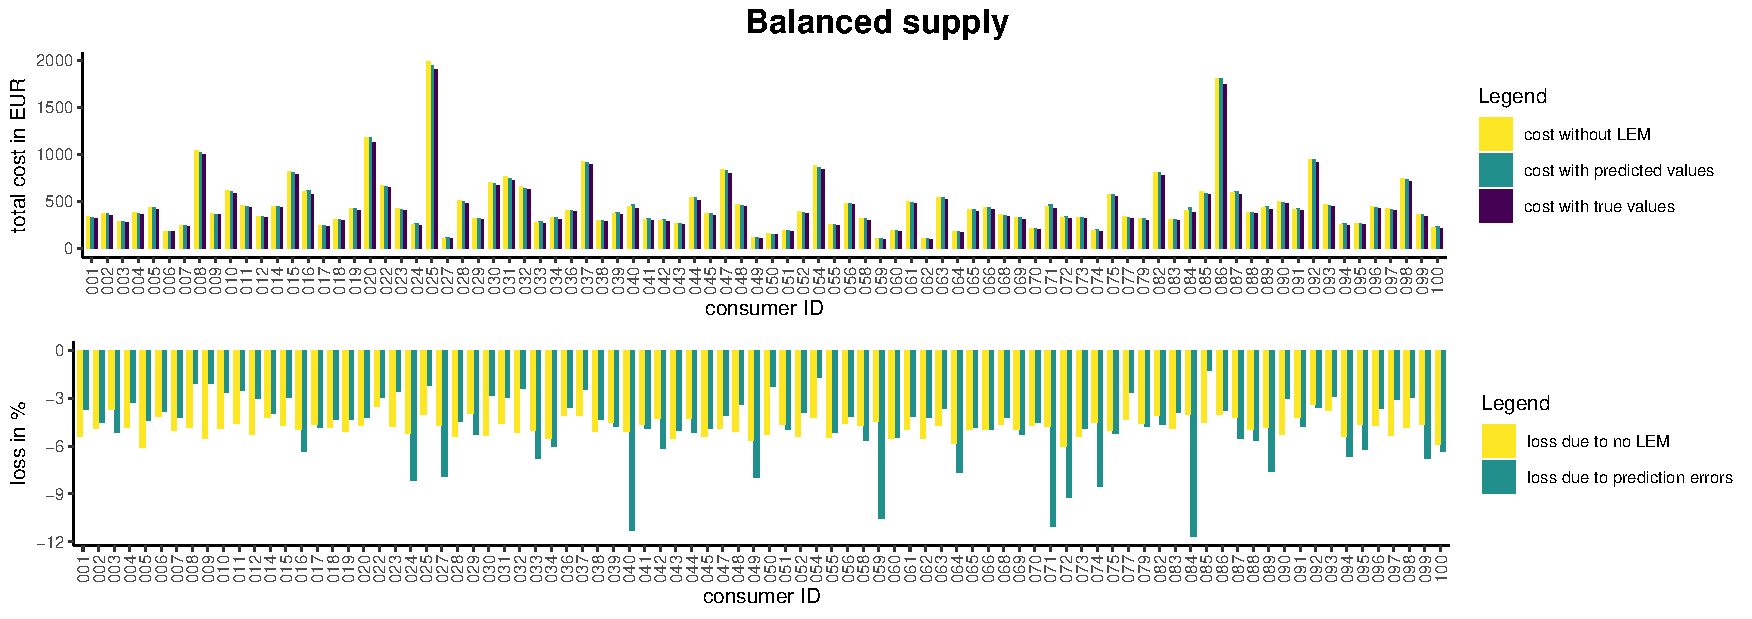
\includegraphics[width=\textwidth]{thesis/graphs/marketsimulation/totalenergycost_balanced.pdf}\\\vspace{.6cm}
    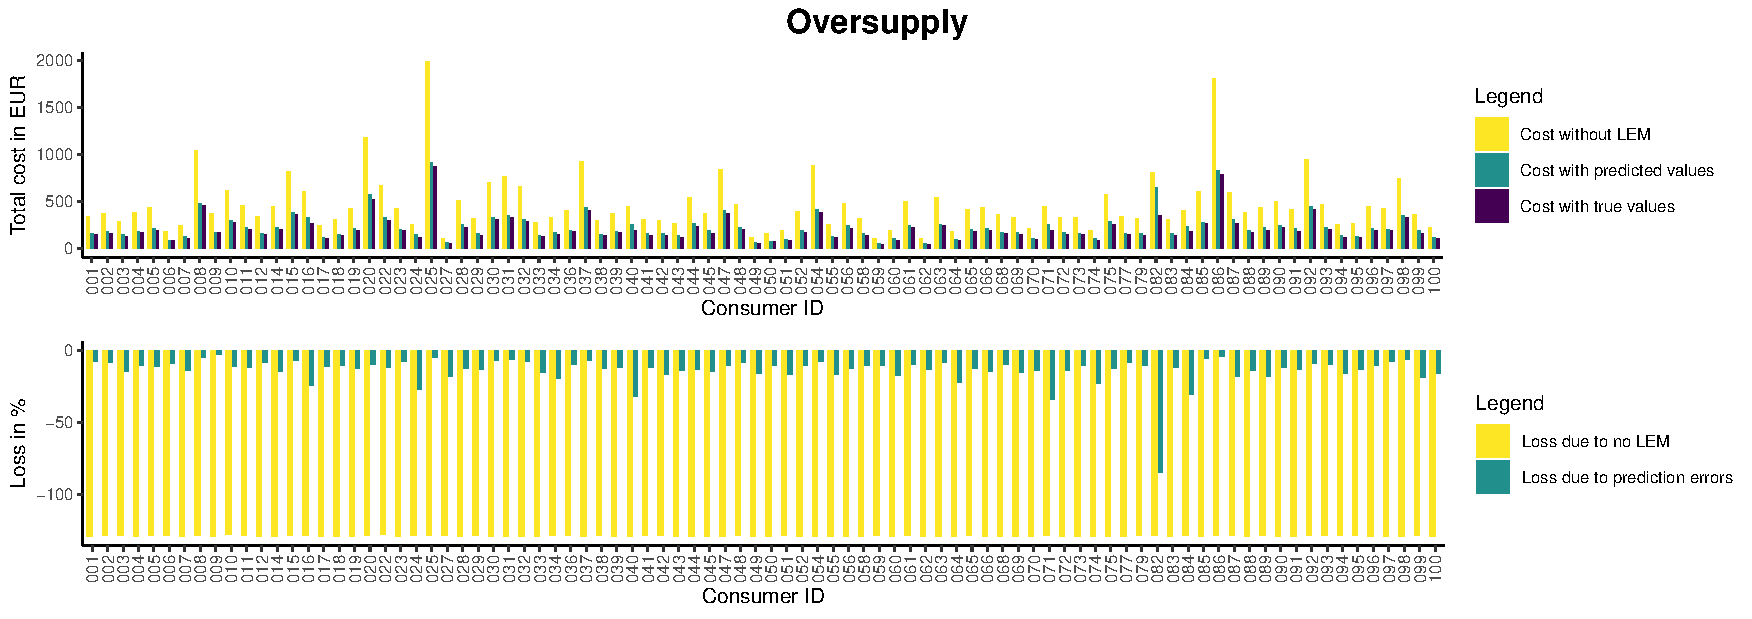
\includegraphics[width=\textwidth]{thesis/graphs/marketsimulation/totalenergycost_oversupply.pdf}\\\vspace{.6cm}
    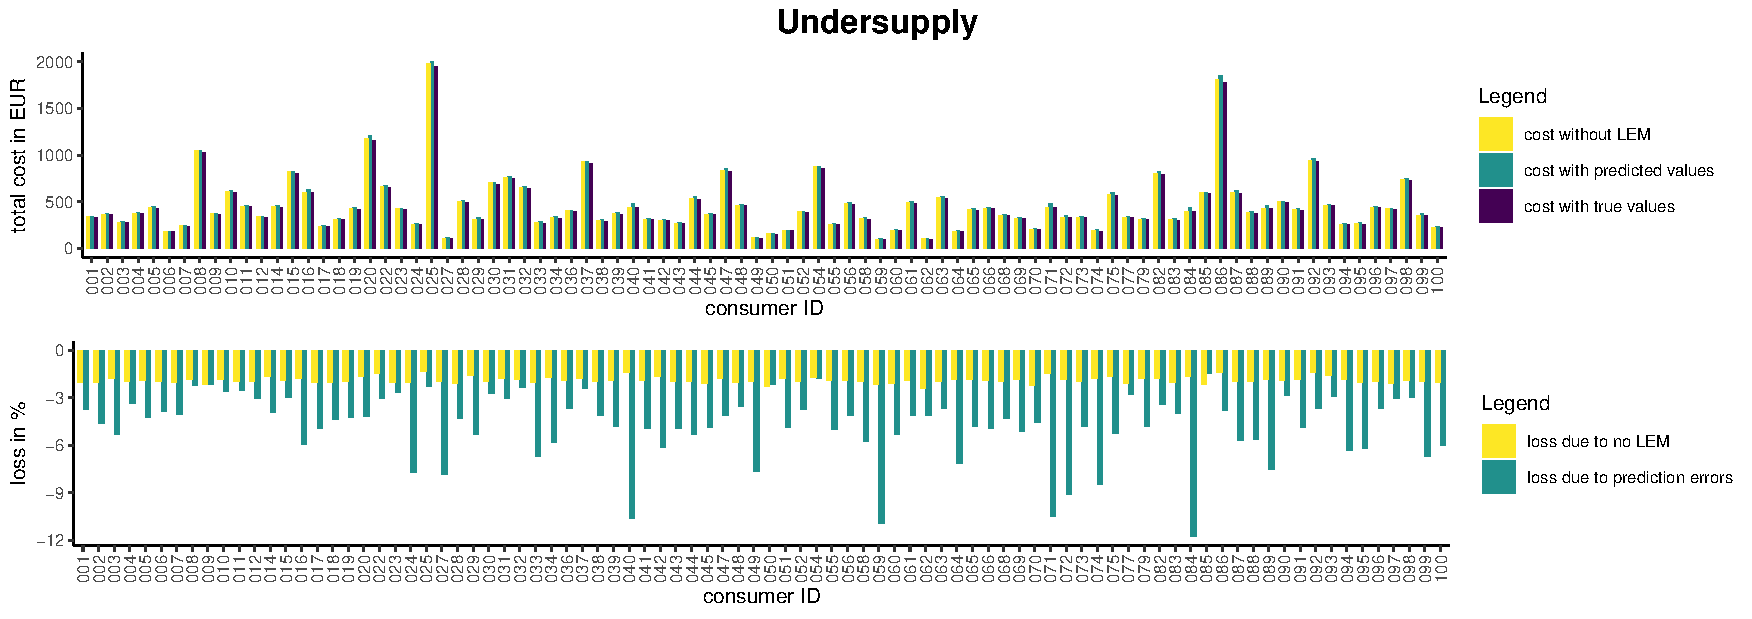
\includegraphics[width=\textwidth]{thesis/graphs/marketsimulation/totalenergycost_undersupply.pdf}
    \caption[Total energy cost to consumers in different supply scenarios]{Total energy cost to consumers from 01.10.2018 to 31.12.2017 in case of no LEM, LEM with true values, and LEM with predicted values in three different supply scenarios. \quantnet\href{https://github.com/QuantLet/BLEM/tree/master/BLEMevaluateMarketSim}{BLEMevaluateMarketSim}}
    \label{Fig:total_energycost}
\end{figure}
%

Overall, it becomes clear that prediction errors significantly lower the economic profitability for consumers. This, however, is often argued to be one of the main advantage of LEMs. The result is especially concerning in LEMs where locally produced energy is undersupplied. Here -- still assuming the closed double auction market mechanism and zero-intelligence bidding strategies -- the savings from the participation in the LEM are marginal. Therefore, the costs induced by prediction errors mostly outweigh the savings from the participation. This results in an overall loss for consumers due to the LEM which makes the participation economically irrational. Only in cases of substantial oversupply, the much lower equilibrium price compared to the energy utility's price compensates for the costs from prediction errors.

In conclusion, this means that LEMs with the market mechanism proposed in \citet{Mengelkamp:2018a} and the prediction accuracy of state-of-the-art energy forecasting techniques require substantial oversupply in the local market for a LEM to be beneficial to consumers.



%%%%%%%%%%%%%%%%%%%%%%%%
%%%   Implications   %%%
%%%%%%%%%%%%%%%%%%%%%%%%

\subsection{Implications for blockchain-based local energy markets}\label{Sec:Results;Subsec:Implications}

In light of these results, it remains open to derive implications and to propose potential adjustments for a smart contract market mechanism. After all, there are substantial advantages of LEMs which have been established in various studies as pointed out in Section~\ref{Sec:Intro;Subsec:Related} and which still make LEMs an attractive solution for the challenges brought about by the changing energy landscape. Adjustments mitigating the negative effect of prediction errors on the profitability of LEMs could address one or more of the following areas: first, the forecasting techniques employed, second, the demand and supply structure of the LEM, and third, the market mechanism used in the blockchain-based LEM.

The first and most intuitive option is to improve the forecasting accuracy with which the predictions, that serve as the basis of bids and asks, are made. The most obvious way to achieve such an improvement is the inclusion of more data. More data may hereby refer either to a higher resolution of recorded consumption respectively production data or to a wider range of data sources such as behavioral data of household members or data from smart appliances. A higher resolution of smart meter readings is already easily achievable. The smart meters installed by Discovergy that also supplied the data for the present research are capable of recording energy measurements up to every two seconds. However, data at such a fine granularity requires substantial data storage and processing capacities which are unlikely to be available in an average household. Especially, the training of prediction models with such vast amounts of input data points is computationally very resource intensive. The potential solution of outsourcing the data processing, the prediction model training, and the prediction making, however, introduces new data privacy concerns that are already a sensible topic within blockchain-based LEMs. \citet{Greveler:2012}, for example, found in 2012 that the data transmitted by Discovergy smart meters to Discovergy servers was not encrypted and easily interceptable. While this is most likely not possible anymore, it exemplifies the general vulnerability of internet-connected systems regarding data protection. Moreover, the authors showed that the data could be used to identify the television program which the household's LCD television was showingwith high precision. This highlights the sensibility of high-resolution energy consumption data as it allows for detailed inference of household members' behavior. The inclusion of behavioral data into prediction models such as the location of the person within their house or apartment and the inclusion of smart appliances' energy consumption (as done by \citet{Kong:2018}) and running schedules raises important privacy concerns as well. Using energy consumption data of several households, as done by \citet{Shi:2017}, again introduces privacy concerns. According to them, the data of several households in a neighborhood could be pooled to utilize common uncertainty within the data for model training and subsequently better prediction for individual households. However, this implies data sharing between households, which in relatively small LEMs cannot be guaranteed to preserve the anonymity of market participants, and thus, is not desirable from a data protection perspective. For all these reasons, it seems unlikely that in the near future much better predictions of the very short-term household energy consumption or production of individual households will be available.

The second option addresses the demand and supply structure in the blockchain-based LEM. As was shown in Section~\ref{Sec:Results;Subsec:Simulation}, the cost induced by prediction errors and their settlement is more than compensated in an oversupply scenario. Hence, employing LEMs only in a regional neighbourhood with energy production that surpasses energy consumption would mitigate the problem of unprofitability due to prediction errors as well. Where this is not possible, participation to the LEM could be restricted such that oversupply in a majority of trading periods is ensured. However, this seems to be an artificial market manipulation that most likely makes most of LEMs' advantages obsolete. Moreover, it is unclear on what basis the restriction to participate in the market should be grounded.

Lastly, the third option to mitigate the problem is the market mechanism and the prediction error settlement structure. A simple approach to reduce forecasting errors is to decrease the forecasting horizon. Thus, instead of having 15-minutes trading periods which also require 15-minutes ahead forecast, the trading periods could be shrunk to just 3 or 1 minute. This would increase the forecasting accuracy, and thereby, lead to lower costs due to the settlement of prediction errors. However, in a blockchain-based LEM more frequent market closings come at the cost of more computational resources needed for transaction verification and cryptographic block generation. Depending on the consensus mechanism used for the blockchain, the energy requirements for the computations that secure transactions and generate new blocks may be substantial. This, of course, is rather detrimental to the idea of promoting more sustainable energy generation and usage. Nevertheless, using consensus mechanisms based on identity verification of the participating agents may serve as a less computational, and thus energy intensive alternative, which might make shorter trading intervals reasonable.

Another, more radical approach might be to change the market mechanism of closed double auctions altogether and use an exposed market instead. Hereby, the energy consumption and production is settled in an auction after the true values are known, instead of in advance. This means, market participants submit just limit prices in their bids and asks without related amounts and the offers are matched in an auction in regular time intervals. Then, the electricity actually consumed and produced in the preceding period is settled according to the market clearing price. Related to this approach is a solution, where bidding is based on forecasted energy values, while the settlement is shifted by one period such that the actual amounts can be used for clearing. This approach, however, may introduce the possibility of fraud and market manipulation as agents can try to deliberately bid using false amounts. While in the smart contracted developed by \citet{Mengelkamp:2018a} funds needed to backup the bid are held as pledges until the contract is settled (this ensures the availability of the necessary funds to pay the bid), this would be senseless, if settlement is only based on actual consumption without considering the amount specified in the offer. However, the extent of this problem and ways to mitigate it should be assessed from a game theoretical perspective that is out of scope of the present research.

All in all, prediction errors have to be taken into account for future designs of blockchain-based LEMs. Otherwise, they may substantially lower the profitability and diminish the incentive to participate in a LEM for consumers. Also, the psychological component of having to rely on an unreliable prediction algorithm that may be more or less accurate depending on the household's energy consumption patterns seems unattractive. Even though possible solutions are not trivial and each come with certain trade-offs, there is room for future improvement of the smart contracts and the market mechanism they reproduce.

%%%%%%%%%%%%%%%%%%%%%%%%%%%%%%%%%%%%%%%%%%%%%%%%%%%%%%%%%%%%%%%%%